\documentclass[10pt,twocolumn,letterpaper]{article}

\usepackage{cvpr}
\usepackage{times}
\usepackage{epsfig}
\usepackage{graphicx}
\usepackage{amsmath}
\usepackage{amssymb}
\usepackage{caption}
\usepackage{subcaption}
\usepackage{float}

% Include other packages here, before hyperref.

% If you comment hyperref and then uncomment it, you should delete
% egpaper.aux before re-running latex.  (Or just hit 'q' on the first latex
% run, let it finish, and you should be clear).
\usepackage[breaklinks=true,bookmarks=false]{hyperref}

\cvprfinalcopy % *** Uncomment this line for the final submission

\def\cvprPaperID{****} % *** Enter the CVPR Paper ID here
\def\httilde{\mbox{\tt\raisebox{-.5ex}{\symbol{126}}}}

% Pages are numbered in submission mode, and unnumbered in camera-ready
%\ifcvprfinal\pagestyle{empty}\fi
\pagenumbering{gobble}
\begin{document}

%%%%%%%%% TITLE
\title{Image Quilting for Texture Synthesis and Transfer}

\author{Aman Kansal\\
170050027\\
\and
Ansh Khurana\\
170050035\\
\and
Kushagra Juneja\\
170050041
}

\maketitle
%\thispagestyle{empty}

% %%%%%%%%% ABSTRACT
% \begin{abstract}
   
% \end{abstract}

%%%%%%%%% BODY TEXT
\section{Introduction}
We present a simple method which given a texture image, generates new images having the same texture. We do this by stitching together small patches of the texture image to generate a new image having same texture. We also extend the algorithm to perform texture transfer i.e. rendering an object with the texture taken from a different object. Unlike other methods which use one-pixel-at-a-time synthesis, our method uses patches of the image at a time and hence provides a great computational advantage while not compromising with the results since even in complicated textures as well the degree of freedom is only of a few pixels and hence patches are an intuitive choice. 
% \begin{figure}[h]
% \begin{center}
% 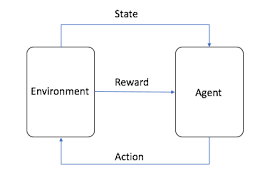
\includegraphics[scale=0.50]{resources/rl_general.png}
% \end{center}
% \vspace{-0.2em}
% \caption{Reinforcement Learning Paradigm}
% \label{fig:basic}
% \end{figure}
%-------------------------------------------------------------------------
\vspace{-6pt}
\section{Method}

\subsection{Quilting}
The patch-based synthesis algorithm in this approach picks small blocks from the texture image and stitches them together to form a larger image that follows the same texture. This algorithm is similar to the quilting procedure used in textile where pieces of fabric are stitched together using a needle and thread.
\subsubsection{Algorithm}
\begin{itemize}
\item We construct the image to be synthesized in units of a block. 
\item For every location, we search the input texture and find the set of blocks which match the above and the left block in the overlapping region. Precisely, we choose those blocks whose error (using L2 norm) with the already placed blocks in the overlapping region are within some tolerance (set to 0.1) of the minimum error. Among these blocks we choose a block randomly.
\item Now, we need to stitch this block with the already placed blocks. To do that, we find the optimal boundary path which minimizes the sum of errors along the path. This is done by dynamic programming. This boundary is visualized in figure \ref{fig:bcut_example}. To the right and bottom of this boundary, we choose the pixels of the new block, and in the other region, we choose the pixels of the old blocks.
\end{itemize}
One hyperparameter is the block size B, that has to be tuned separately for all images. In all experiments, the width of the overlapping region was taken to be 1/3 of block size.
\begin{figure}[h]
\begin{center}
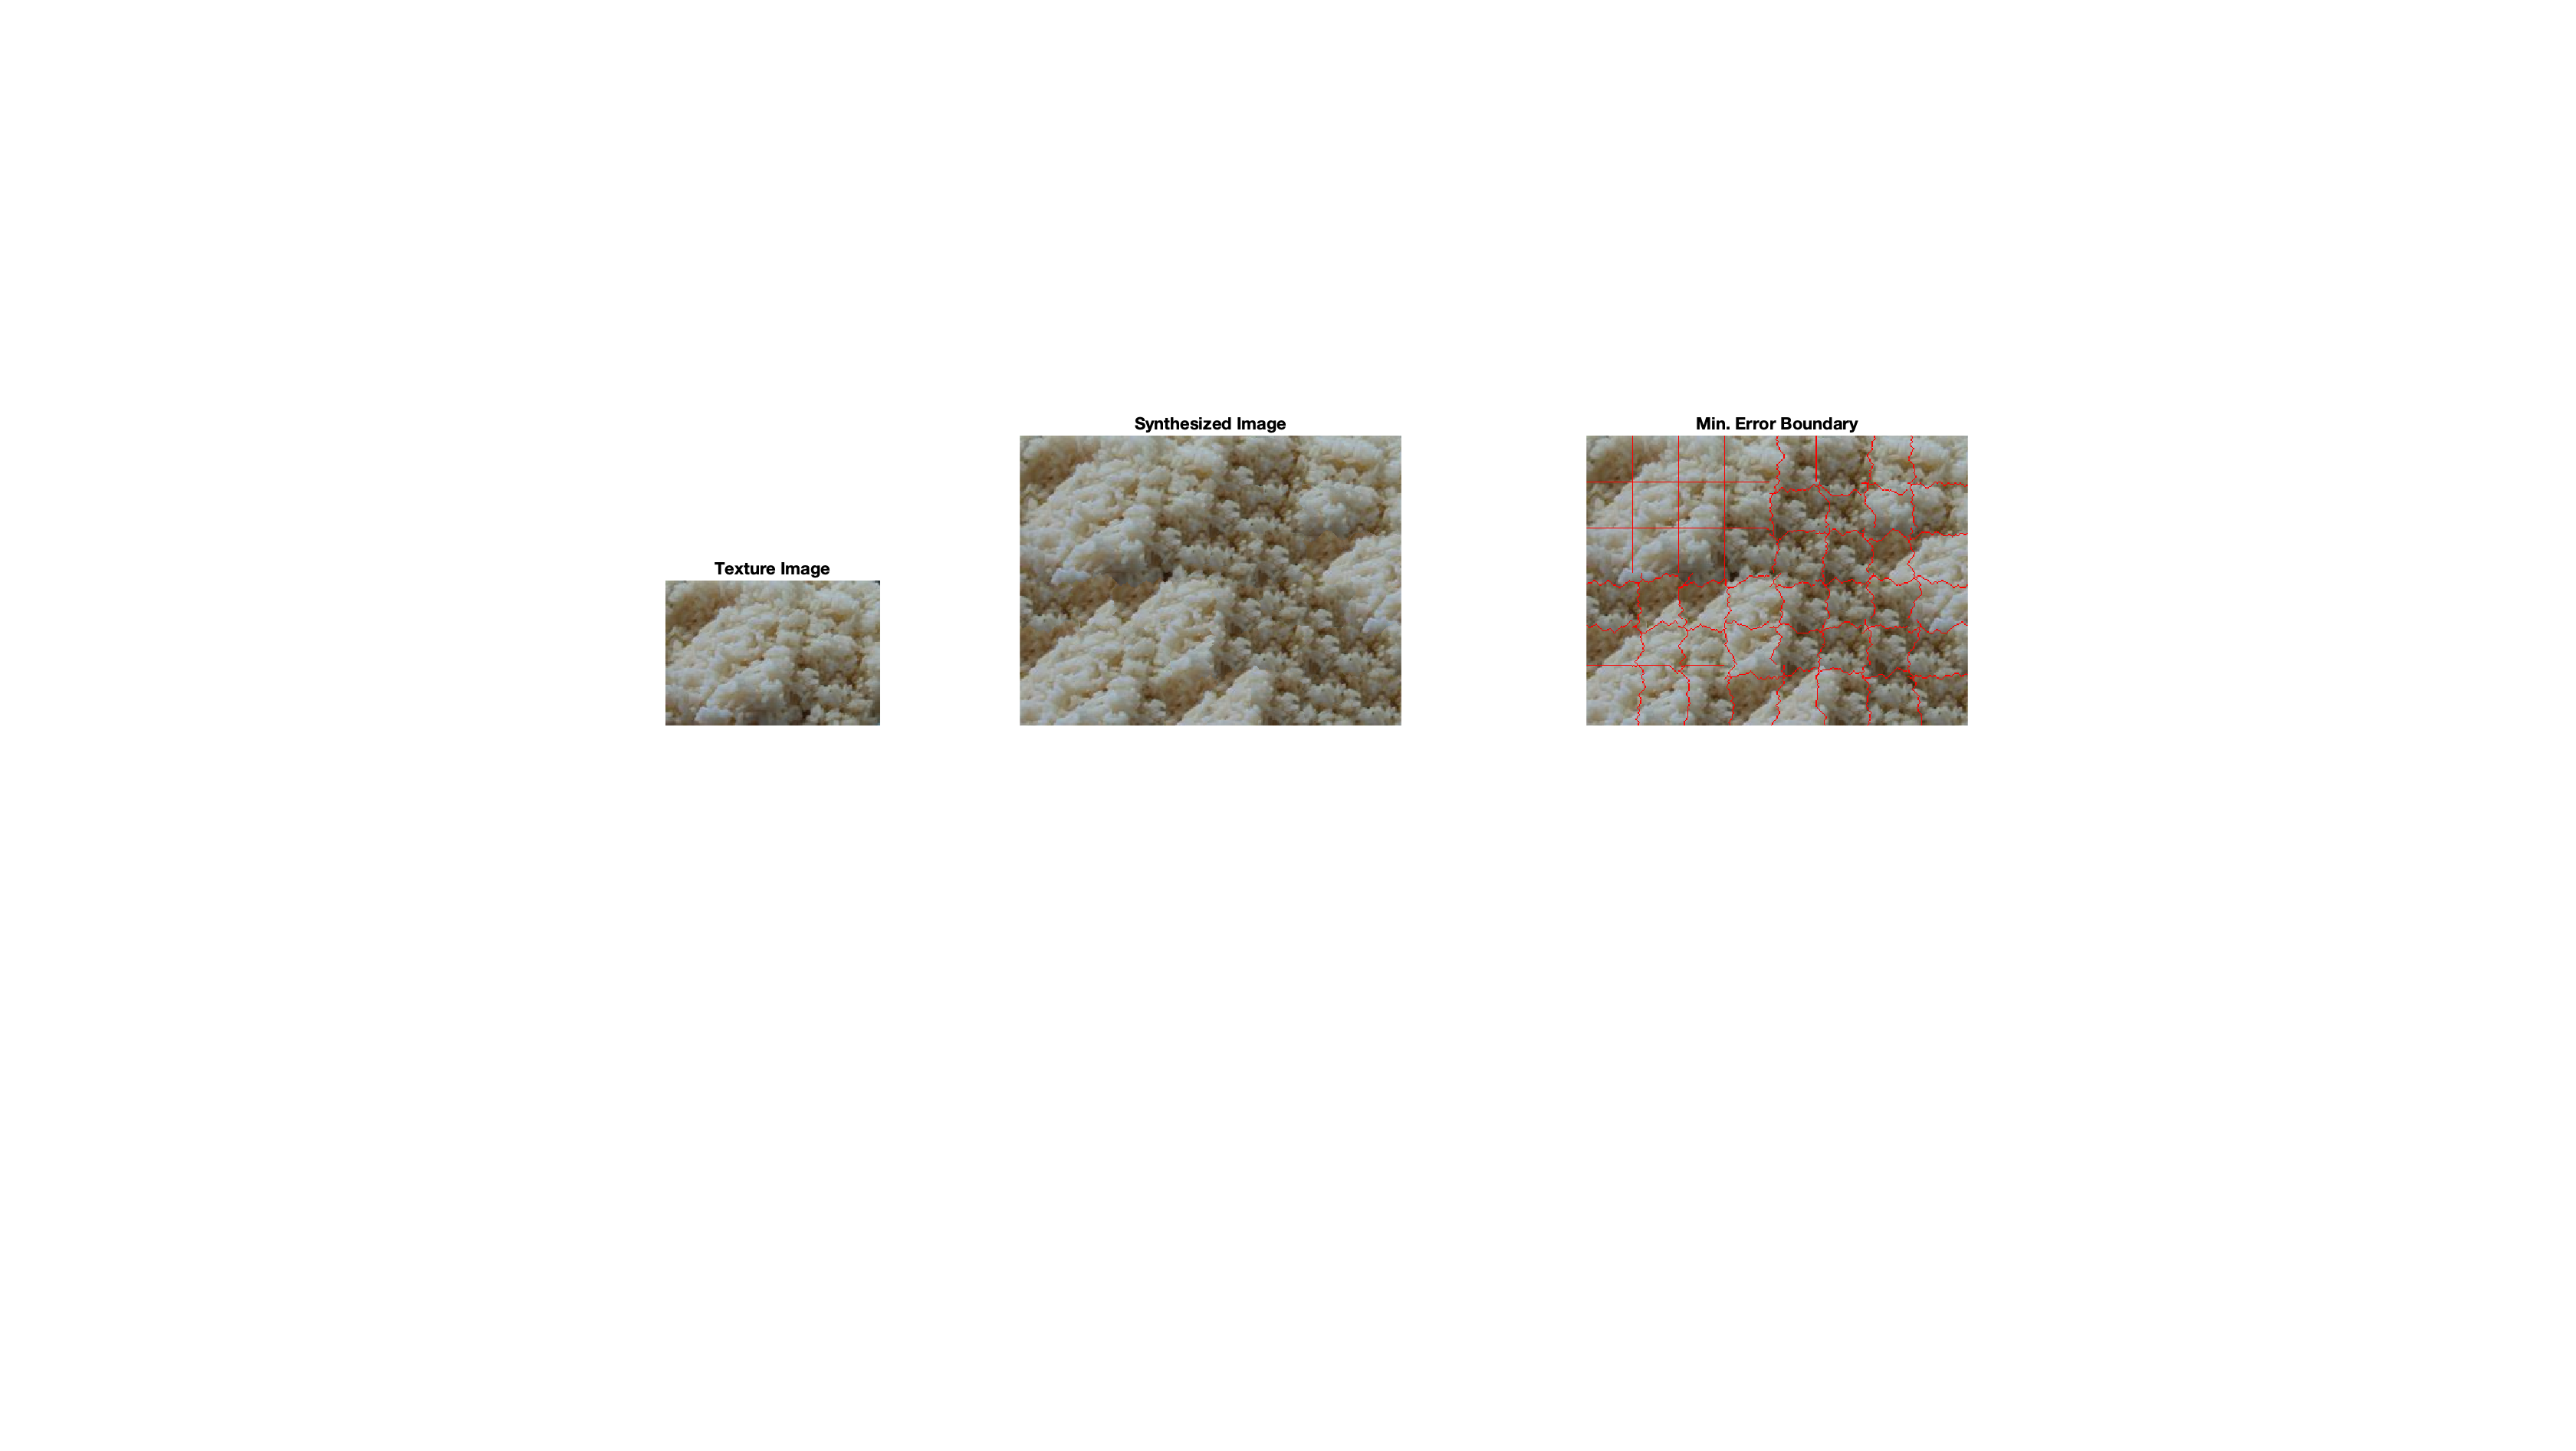
\includegraphics[trim={32cm 34cm 28cm 18cm},clip, scale=0.16]{../rice_boundary_example.png}
\end{center}
\vspace{-0.2em}
\caption{Boundary Cuts in Synthesis of Apple image}
\label{fig:bcut_example}
\end{figure}
% \begin{align*}
%     Q_{n}(s, a) = \left(1-\alpha_{n}\right) Q_{n-1}(s, a)+\alpha_{n}\left[r_{n}+\gamma V_{n-1}\left(y_{n}\right)\right]
% \end{align*}
%-------------------------------------------------------------------------
\subsection{Texture Transfer}
In the task of texture transfer, the input is taken in form
of small piece of texture and a target image. The aim is to
reconstruct the target image from small patches of the given
texture so that the high level information in the image is
preserved while giving it a textured appearance similar to
the input texture.

\subsubsection{Algorithm}
The algorithm for this task is similar to the quilting algo-
rithm, except that the final image is constructed in multiple
iterations, each producing a better output image than the
previous one. The output image is of the same dimensions
as the input target image. Thus, each patch in the output im-
age corresponds to a patch in the target image. After placing
the first patch (at the top-left corner say) in the output im-
age, we progressively place the next patch, stochastically
minimizing the summation of following two losses -

\begin{itemize}
    \item SSE (sum of squared errors) between the pixels in the
    new patch and those in the surrounding patches, in the
    overlap region. Call it SSE1
    \item SSE between the pixels in the new patch and the pixels
    in the corresponding patch of the target image. Call it
    SSE2
\end{itemize}
% \newline
Mathematically the minimized loss is -
\begin{align}
L = \alpha *SSE1 + (1 - \alpha) *SSE2\notag
\end{align}
The paramter $\alpha$, in i th iteration is heuristically kept
as $\alpha_i = 0.8*\frac{i-1}{N-1}+0.1$
where $N$ is the total number
of iterations and is ideally kept between 3 to 5. The size
of the patch is also reduced in each successive iteration
in a geometric fashion, i.e., $B_{i+1} = B_i *d$ where $d$ is
the decay rate for patch size and a hyperparameter for
the algorithm. In the successive iteration we replace the
target image by the image obtained in the previous iteration.
\newline
\newline
\textbf{Intuition behind iterative algorithm} We can observe
that in the successive iterations, in addition to reducing
the patch size, we alter the relative weights for the two
SSE’s adding more weight to maintaining continuity
accross edges. The explanation behind it is as follows -
We choose larger patches first (although still small enough
to be able to replicate target image), so as to preserve the
important components in the texture. This might reflect
some discountinuities at the edges of the block. In the
subsequent iterations, when smaller patches are being
chosen then the patches inside the previously larger patch
would tend to remain same (as they match the target imageperfectly and are inherently continuous), but the patches at
the boundary would be chosen so as the remain closer to
the previously chosen patch, while enhancing continuity
accross the boundary.
%-------------------------------------------------------------------------

\section{Results}
We show some amazing synthesis results below followed by transfer results. 
The results demonstrate the effectiveness of our implementation. The images produced are high quality and realistic for both synthesis and transfer tasks. 
We are able to reproduce results similar in quality when compared to the ones presented in the paper.

\begin{figure*}[!htb]
     \centering
     \begin{subfigure}[h]{0.33\textwidth}
         \centering
         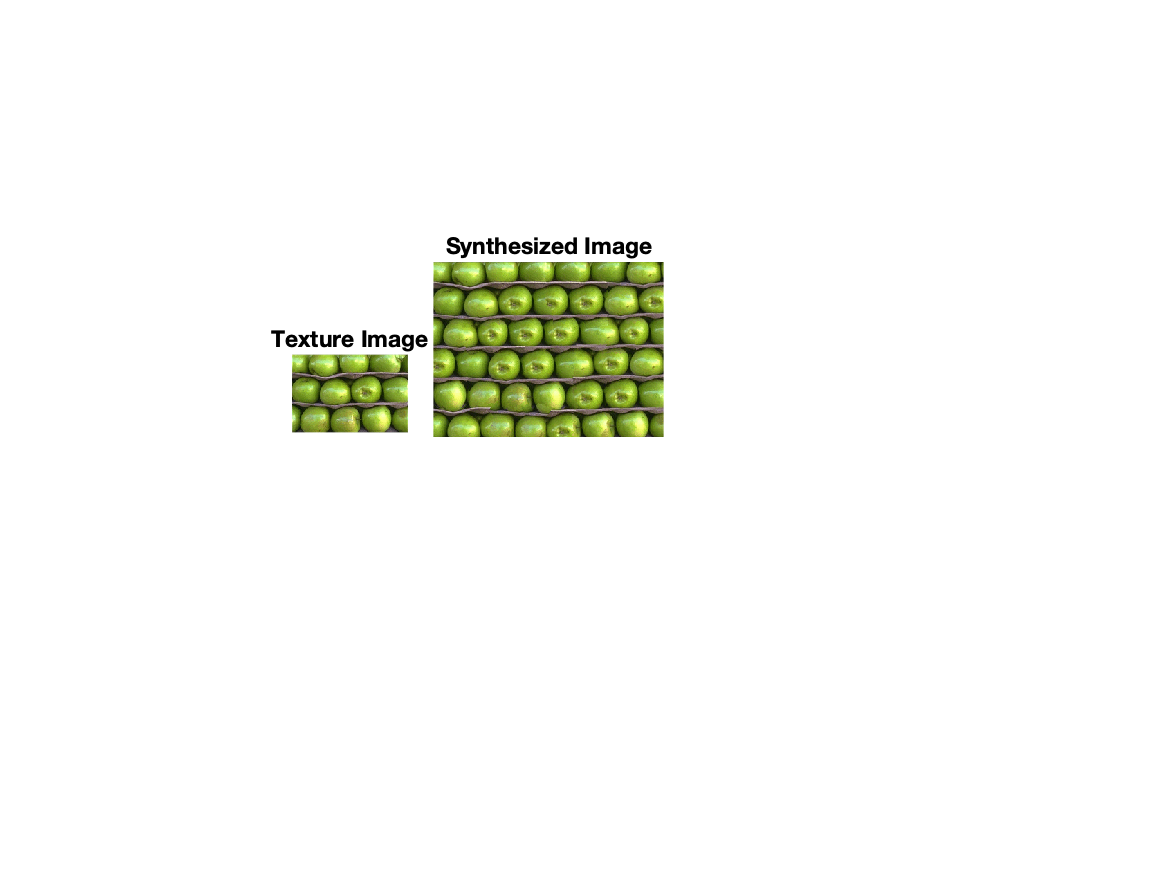
\includegraphics[trim={4.5cm 7cm 8.0cm 3cm}, clip, scale=1.5, width=\textwidth]{../results/syn_final/result_apples_c_B_40.png}
         \caption{Apples}
         \label{fig:apples_res}
     \end{subfigure}
     \hfill
     \begin{subfigure}[h]{0.33\textwidth}
        \centering
        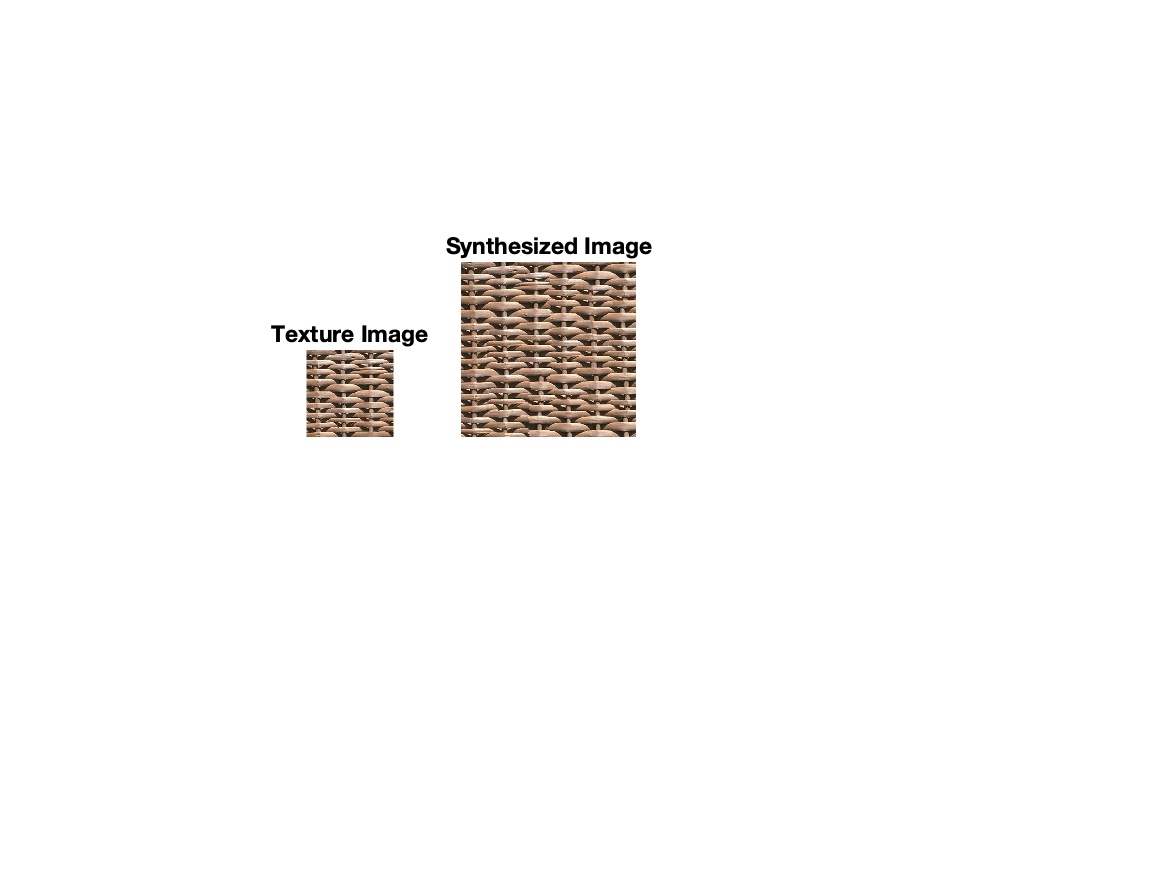
\includegraphics[trim={4.5cm 7cm 8.0cm 3cm}, clip, scale=1.5, width=\textwidth]{../results/syn_final/result_jute_c_B_40.png}
        \caption{Jute}
        \label{fig:jute_res}
    \end{subfigure}
    \hfill
    \begin{subfigure}[h]{0.33\textwidth}
        \centering
        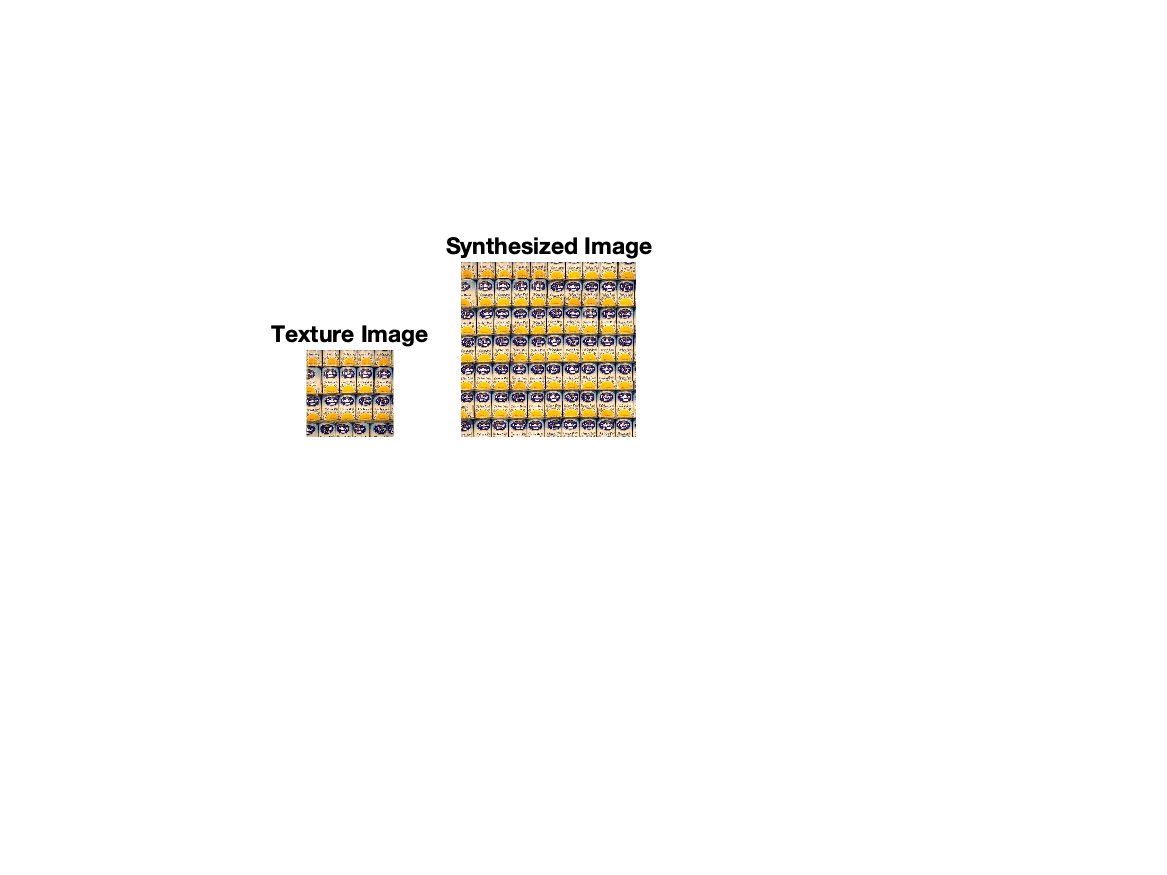
\includegraphics[trim={4.5cm 7cm 8.0cm 3cm}, clip, scale=1.5, width=\textwidth]{../results/syn_final/result_cans_B_80.png}
        \caption{Cans}
        \label{fig:cans_res}
    \end{subfigure}
    \begin{subfigure}[h]{0.33\textwidth}
        \centering
        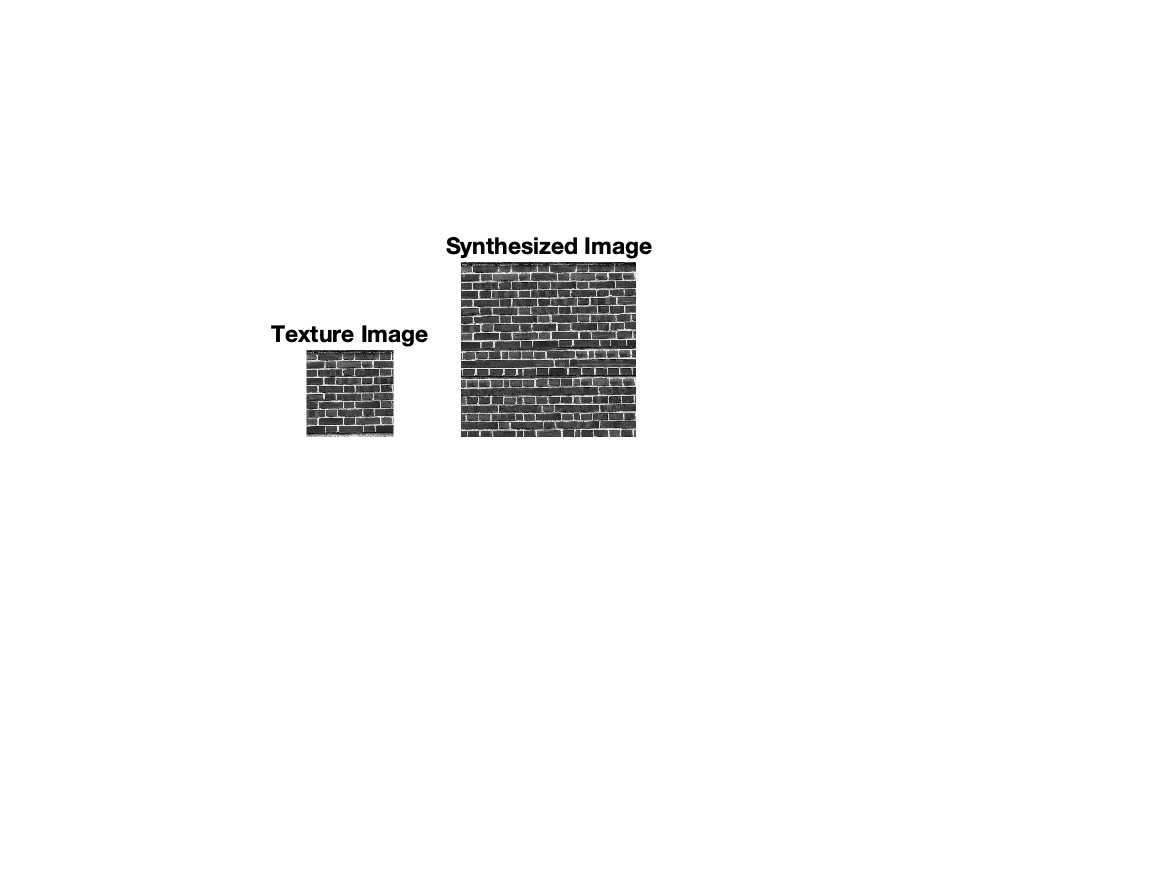
\includegraphics[trim={4.5cm 7cm 8.0cm 3cm}, clip, scale=1.5, width=\textwidth]{../results/syn_final/result_brick_bw_B_40.png}
        \caption{D1}
        \label{fig:d1_res}
    \end{subfigure}
    \hfill
    \begin{subfigure}[h]{0.33\textwidth}
       \centering
       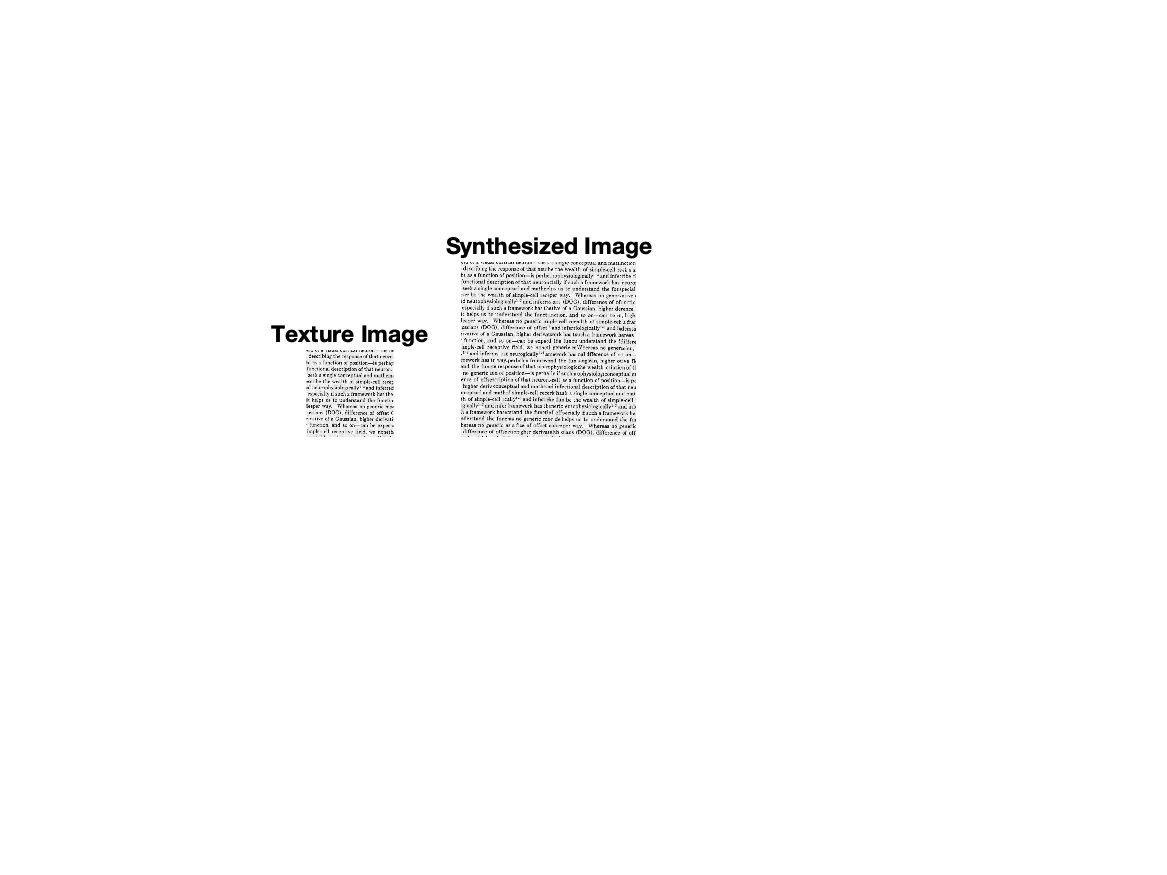
\includegraphics[trim={4.5cm 7cm 8.0cm 3cm}, clip, scale=1.5, width=\textwidth]{../results/syn_final/result_text_B_40.png}
       \caption{text}
       \label{fig:text_res}
   \end{subfigure}
   \hfill
   \begin{subfigure}[h]{0.33\textwidth}
       \centering
       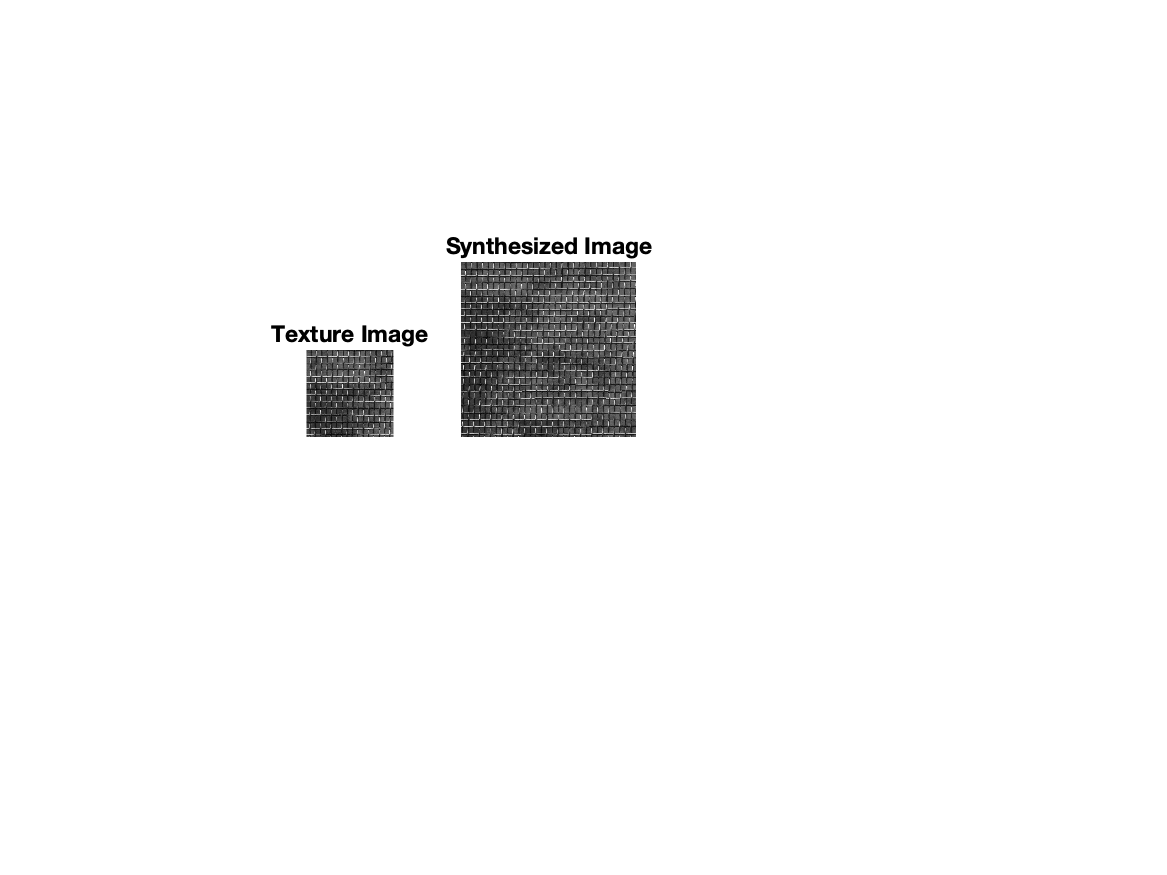
\includegraphics[trim={4.5cm 7cm 8.0cm 3cm}, clip, scale=1.5, width=\textwidth]{../results/syn_final/result_D1_B_40.png}
       \caption{Bricks B/W}
       \label{fig:bricksbw_res}
   \end{subfigure}
   \begin{subfigure}[h]{0.33\textwidth}
         \centering
         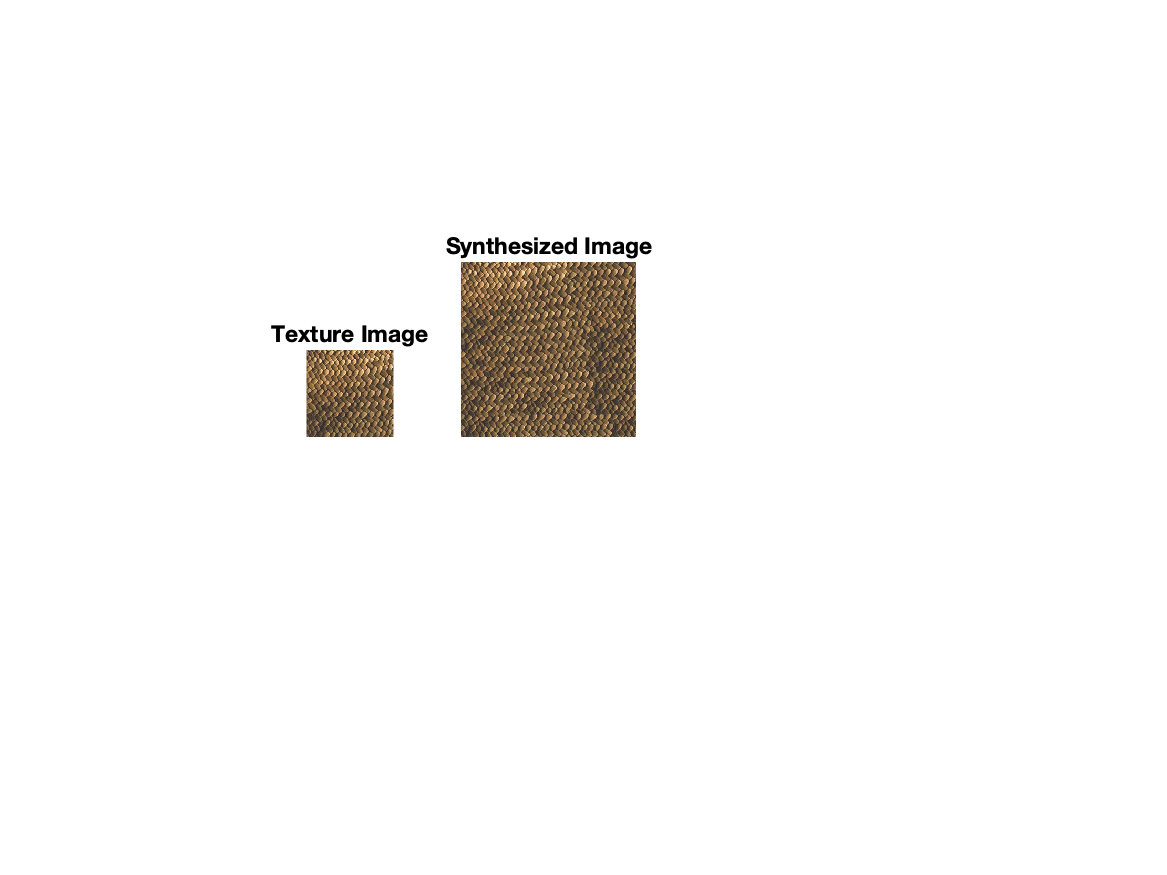
\includegraphics[trim={4.5cm 7cm 8.0cm 3cm}, clip, scale=1.5, width=\textwidth]{../results/syn_final/result_fabric_B_40.png}
         \caption{Fabric}
         \label{fig:apple_res}
     \end{subfigure}
     \hfill
     \begin{subfigure}[h]{0.33\textwidth}
        \centering
        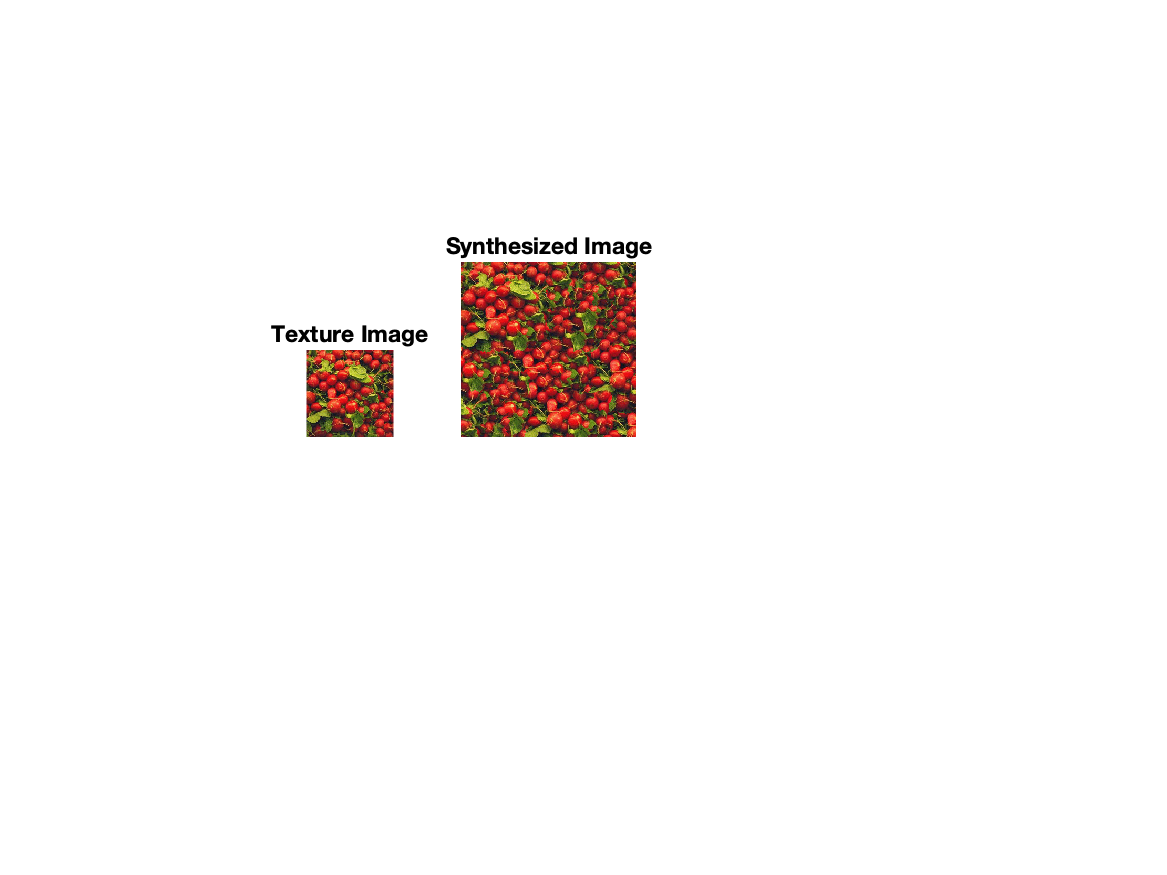
\includegraphics[trim={4.5cm 7cm 8.0cm 3cm}, clip, scale=1.5, width=\textwidth]{../results/syn_final/result_radishes_B_40.png}
        \caption{Radishes}
        \label{fig:apple_res}
    \end{subfigure}
    \hfill
    \begin{subfigure}[h]{0.33\textwidth}
        \centering
        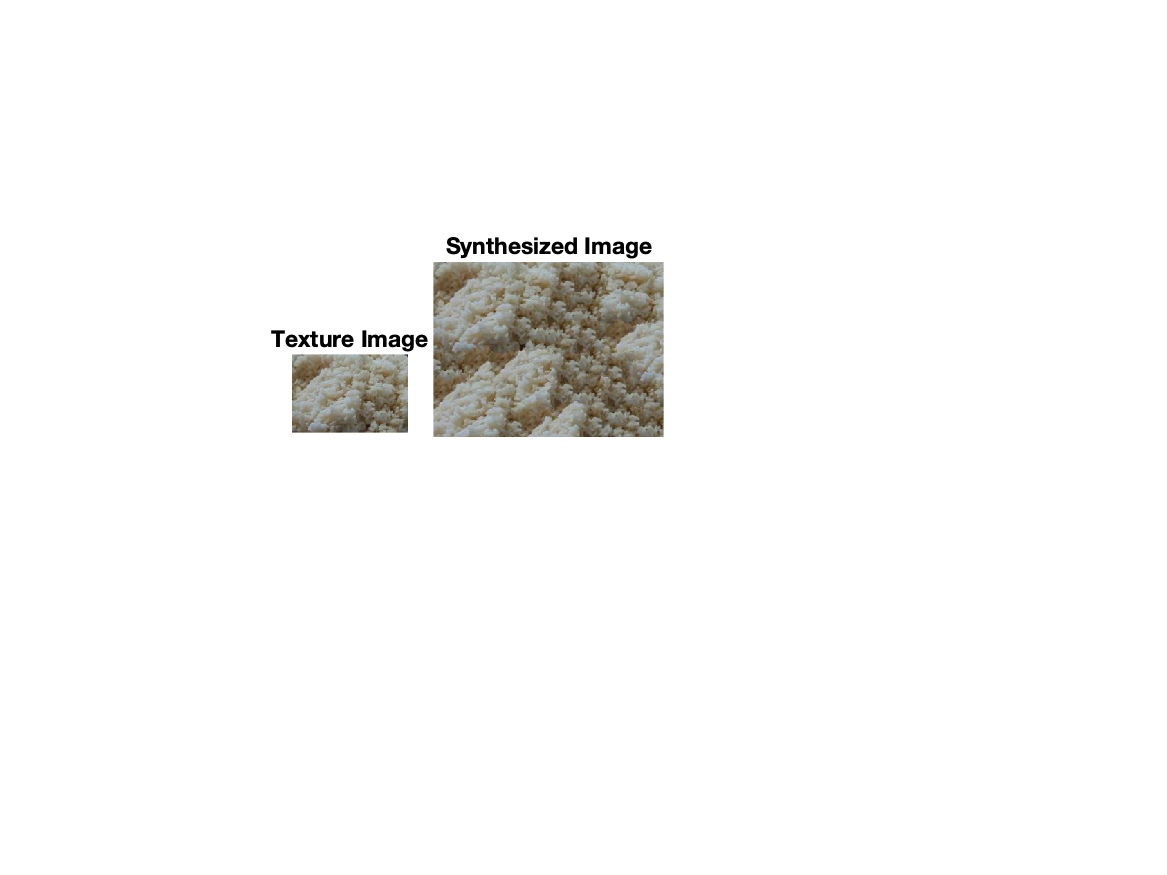
\includegraphics[trim={4.5cm 7cm 8.0cm 3cm}, clip, scale=1.5, width=\textwidth]{../results/syn_final/result_rice_B_40.png}
        \caption{Rice}
        \label{fig:apple_res}
    \end{subfigure}
    \begin{subfigure}[h]{0.33\textwidth}
        \centering
        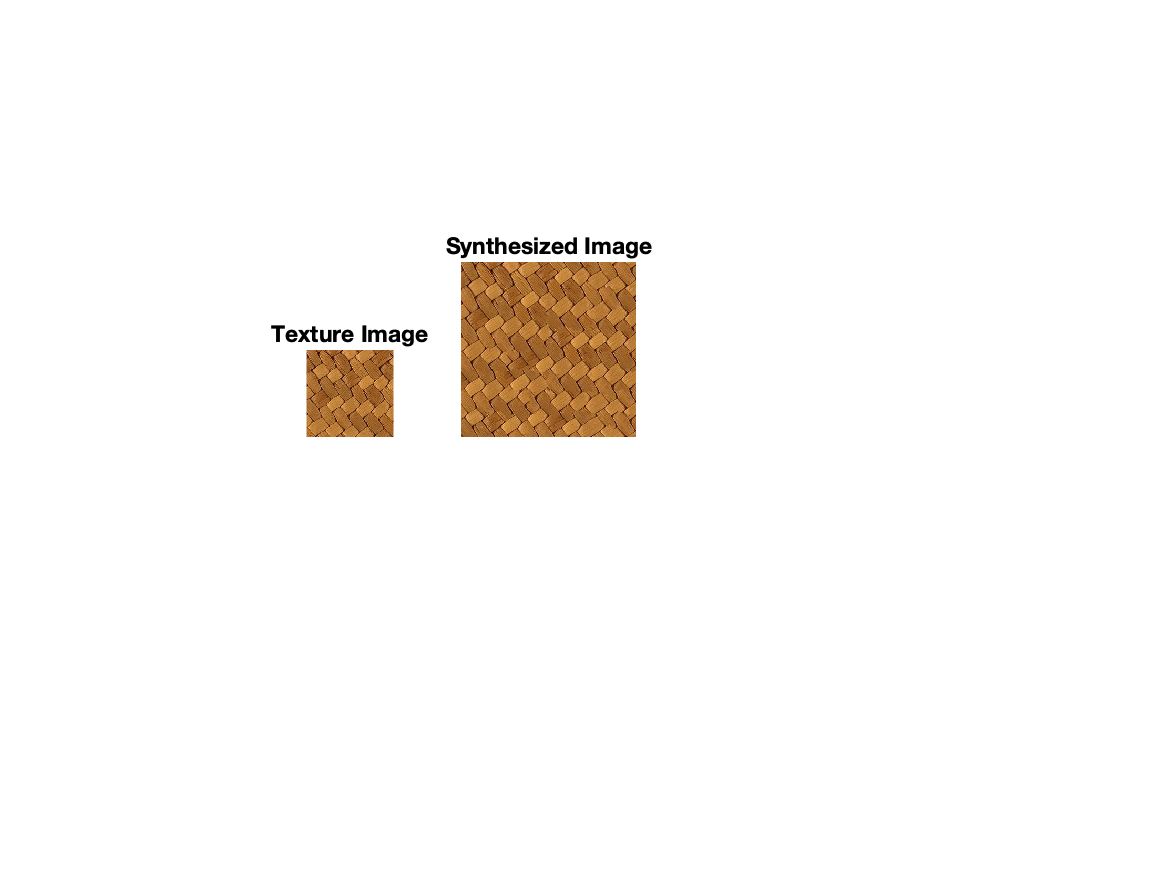
\includegraphics[trim={4.5cm 7cm 8.0cm 3cm}, clip, scale=1.5, width=\textwidth]{../results/syn_final/result_wood_c_B_40.png}
        \caption{Wood}
        \label{fig:apple_res}
    \end{subfigure}
    \hfill
    \begin{subfigure}[h]{0.33\textwidth}
       \centering
       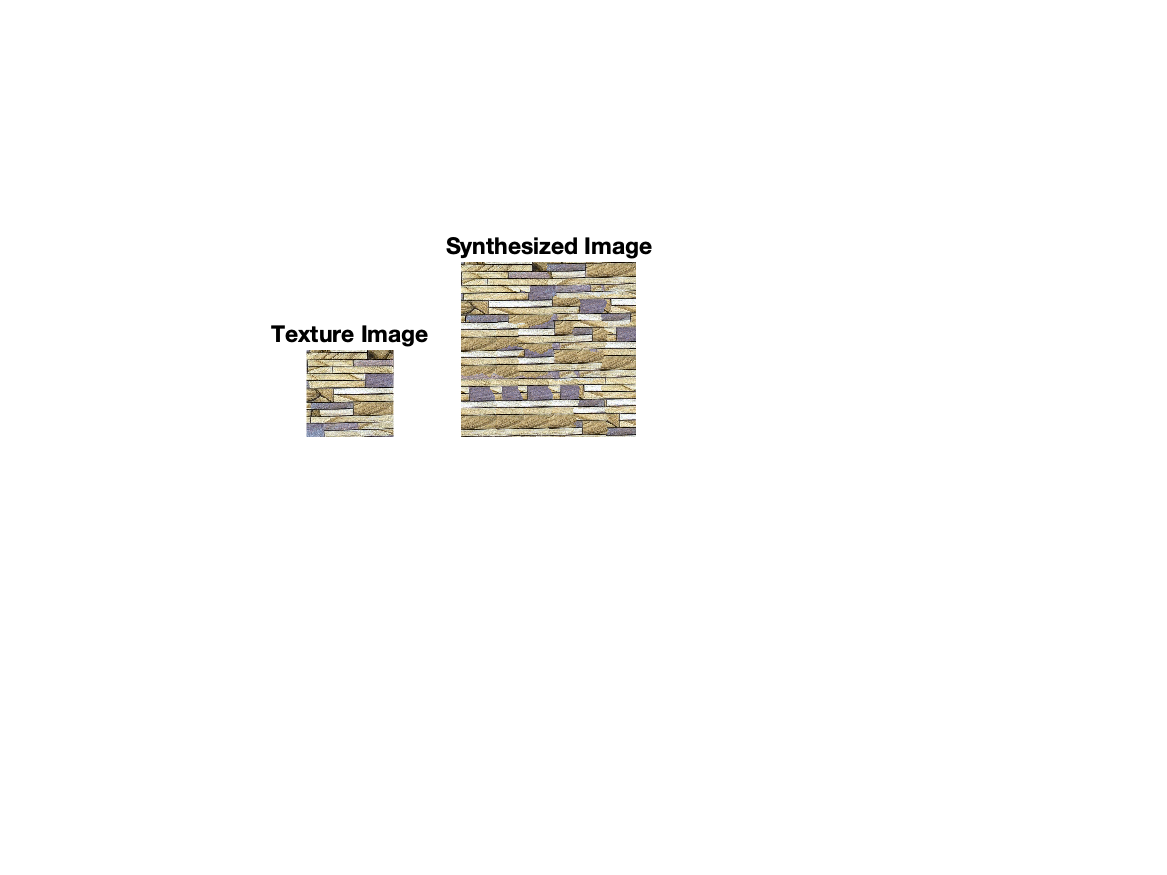
\includegraphics[trim={4.5cm 7cm 8.0cm 3cm}, clip, scale=1.5, width=\textwidth]{../results/syn_final/result_tile_B_60.png}
       \caption{Tiles}
       \label{fig:apple_res}
   \end{subfigure}
   \hfill
   \begin{subfigure}[h]{0.33\textwidth}
       \centering
       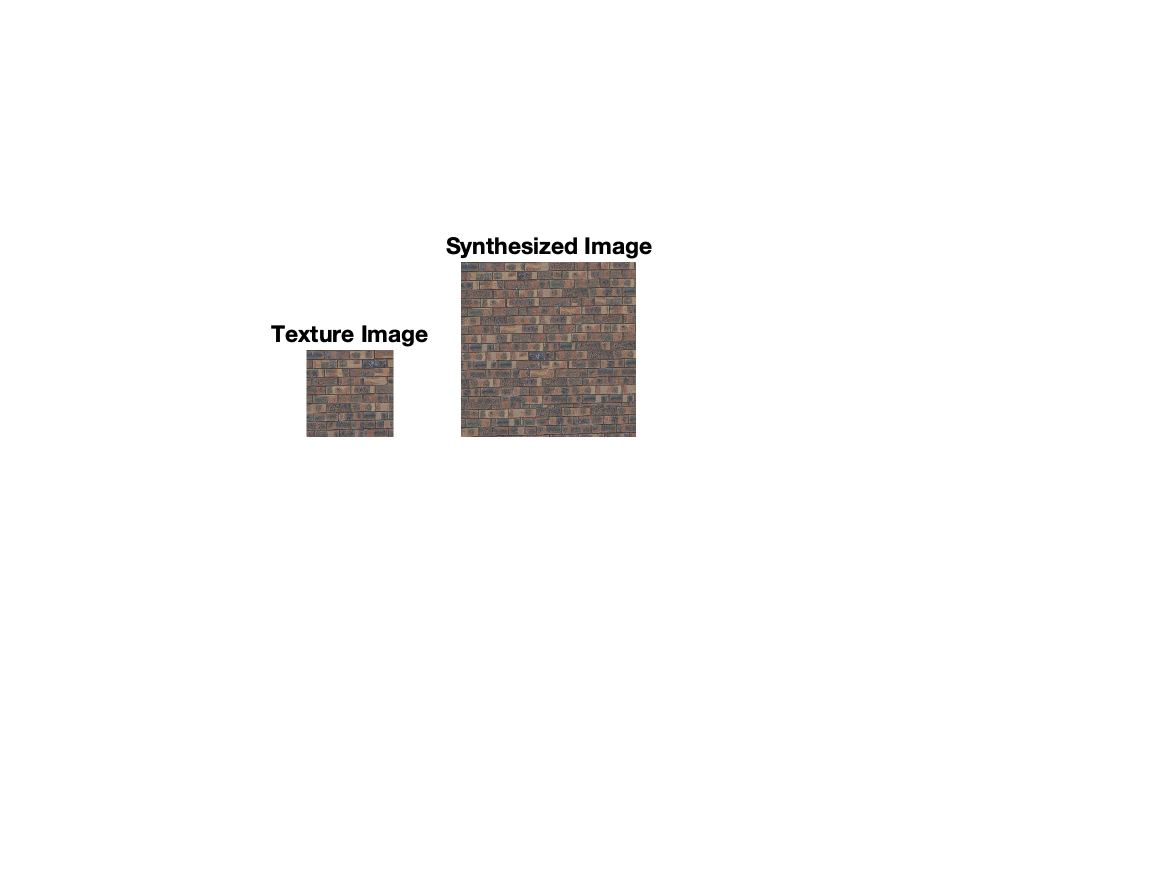
\includegraphics[trim={4.5cm 7cm 8.0cm 3cm}, clip, scale=1.5, width=\textwidth]{../results/syn_final/result_brick_B_60.png}
       \caption{Bricks}
       \label{fig:apple_res}
   \end{subfigure}
   \begin{subfigure}[h]{0.33\textwidth}
    \centering
    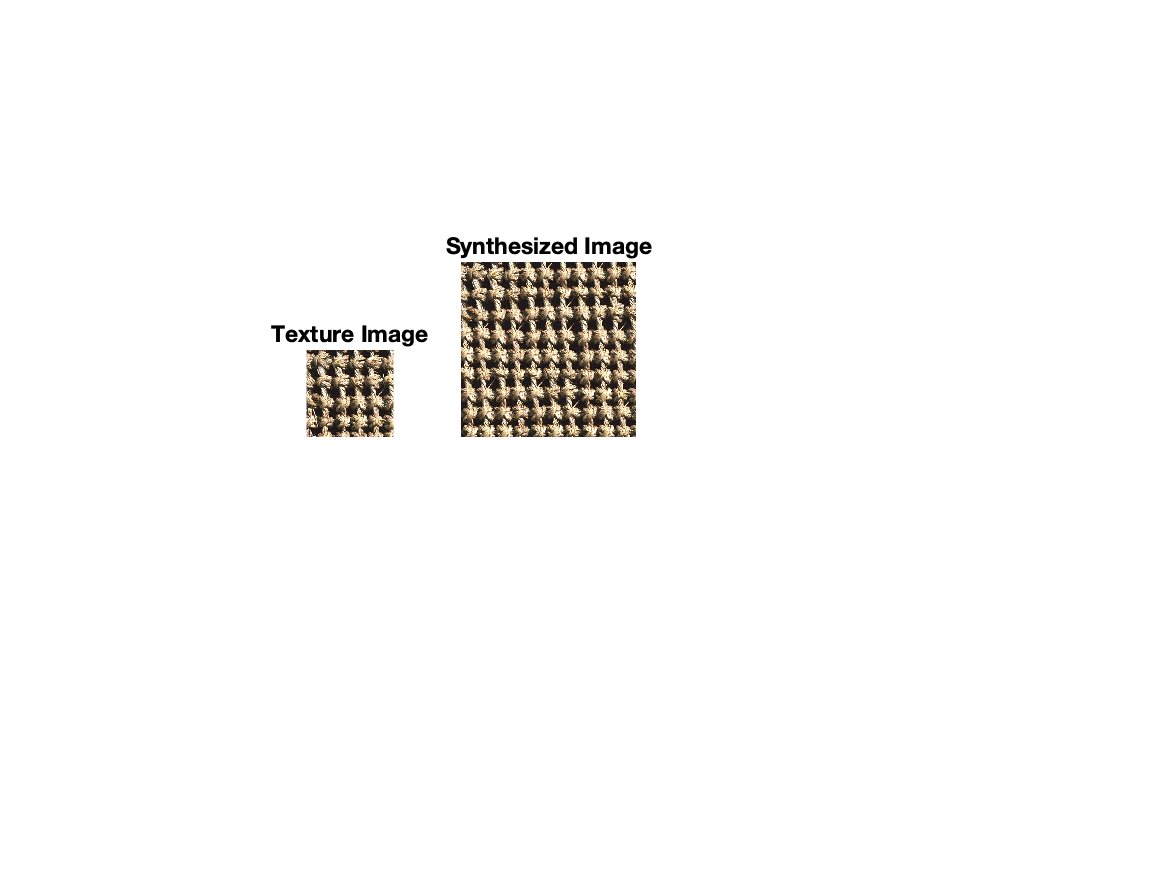
\includegraphics[trim={4.5cm 7cm 8.0cm 3cm}, clip, scale=1.5, width=\textwidth]{../results/syn_final/result_rope_B_60.png}
    \caption{Rope}
    \label{fig:apple_res}
\end{subfigure}
\hfill
\begin{subfigure}[h]{0.33\textwidth}
   \centering
   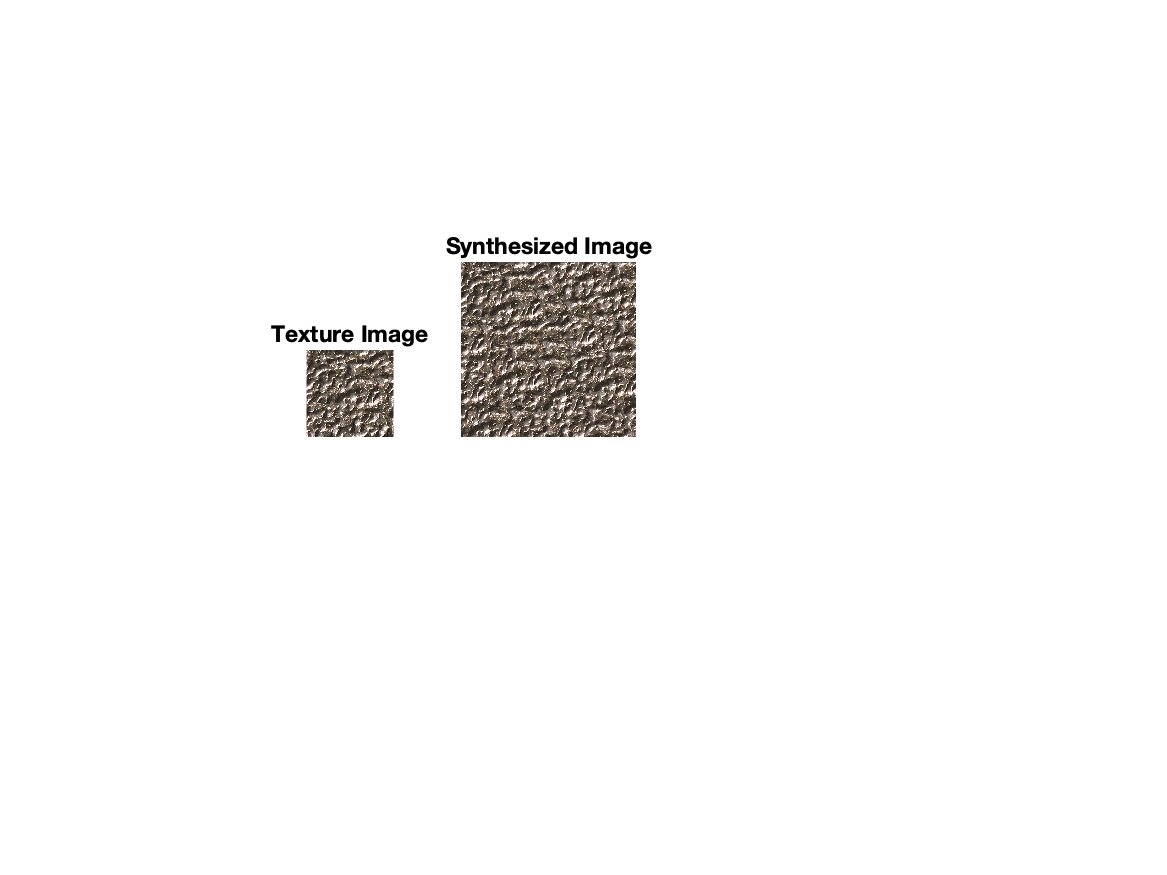
\includegraphics[trim={4.5cm 7cm 8.0cm 3cm}, clip, scale=1.5, width=\textwidth]{../results/syn_final/result_br_pattern_B_60.png}
   \caption{Pattern}
   \label{fig:apple_res}
\end{subfigure}
\hfill
\begin{subfigure}[h]{0.33\textwidth}
   \centering
   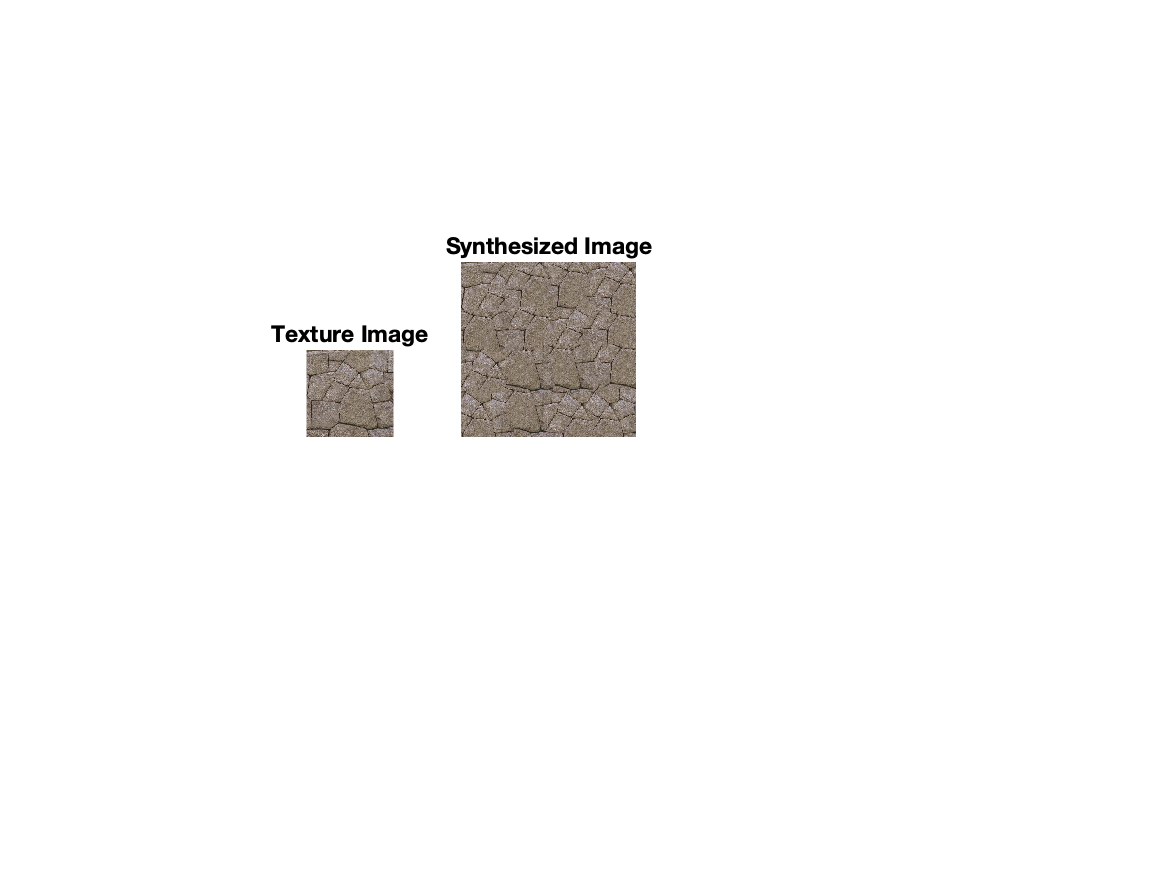
\includegraphics[trim={4.5cm 7cm 8.0cm 3cm}, clip, scale=1.5, width=\textwidth]{../results/syn_final/result_stone_B_90.png}
   \caption{Stone}
   \label{fig:apple_res}
\end{subfigure}   
       \caption{Quilting Results}
        \label{fig:quil_final}
\end{figure*}


\begin{figure*}[h]
    \centering
    \begin{subfigure}[h]{0.4\textwidth}
        \centering
        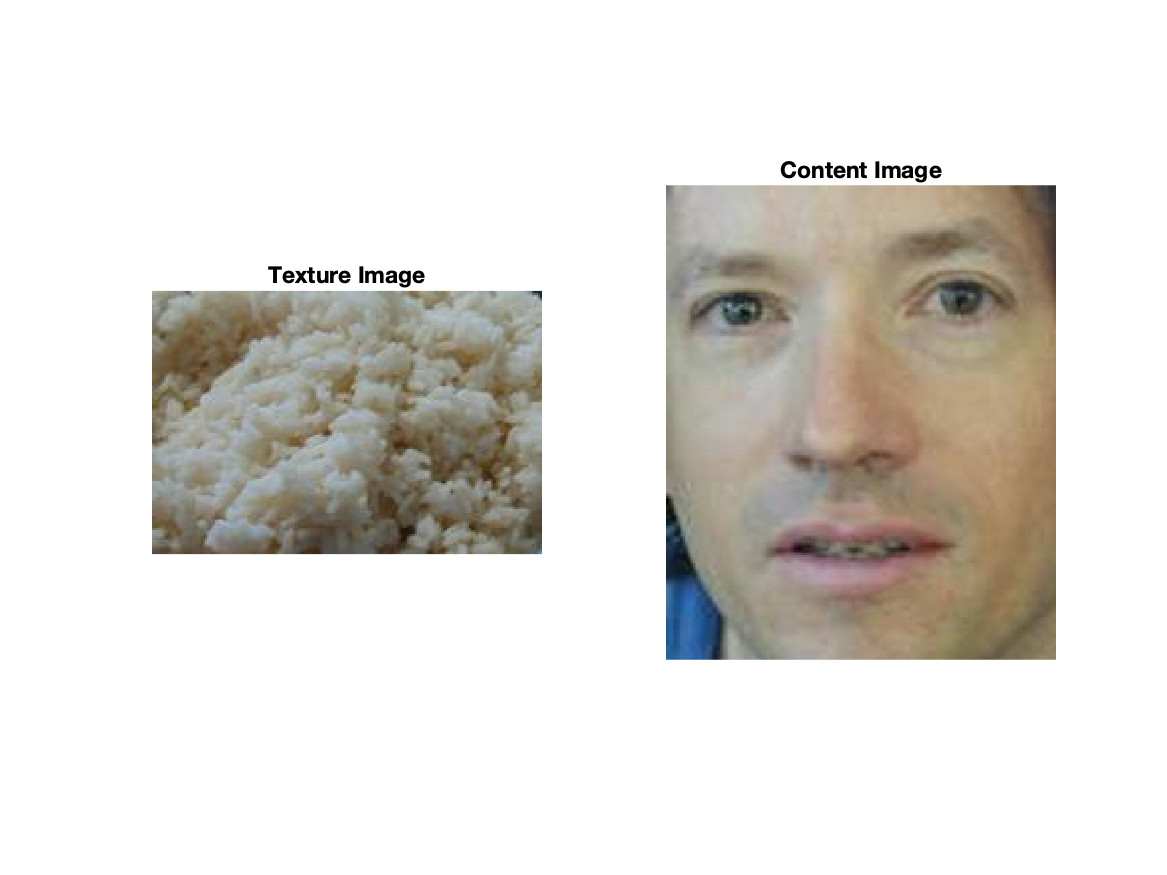
\includegraphics[trim={2cm 4cm 2cm 2cm}, clip, scale=0.5]{../results/bsize/inp_rice_bill.png}
        \caption{Input}
    \end{subfigure}
    \hfill
    \begin{subfigure}[h]{0.5\textwidth}
       \centering
       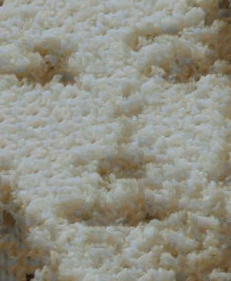
\includegraphics[scale=0.6]{../results/bsize/out_rice_bill_B_20_bdr_0_800000.png}
       \caption{Output}
   \end{subfigure}
   \caption{Result for texture Rice trasferred to Bill image}
   \label{fig:ap_bs}
\end{figure*}

\begin{figure*}[h]
    \centering
    \begin{subfigure}[h]{0.45\textwidth}
        \centering
        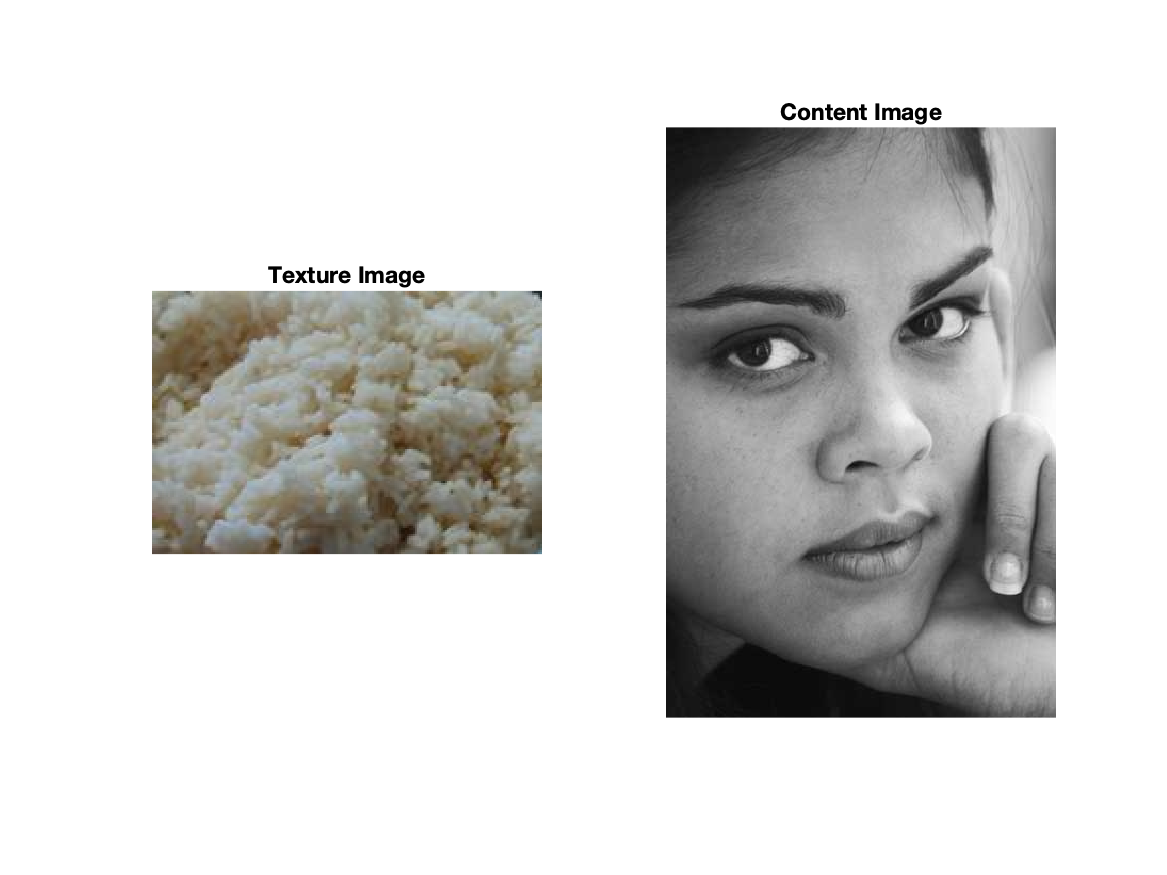
\includegraphics[trim={2cm 4cm 2cm 1cm}, clip, scale=0.5]{../results/bsize/inp_rice_girl.png}
        \caption{Input}
    \end{subfigure}
    \hfill
    \begin{subfigure}[h]{0.5\textwidth}
       \centering
       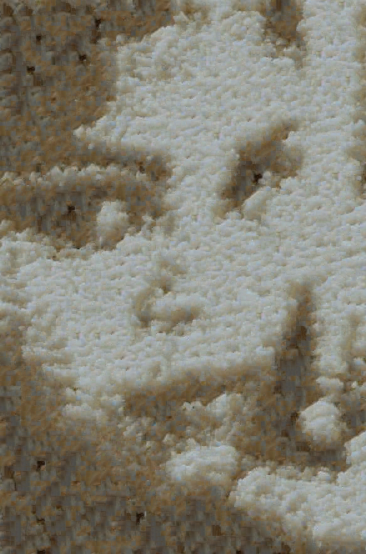
\includegraphics[scale=0.4]{../results/bsize/out_rice_girl_B_20_bdr_0_700000.png}
       \caption{Output}
   \end{subfigure}
   \caption{Result for texture Rice transferred to Girl image}
   \label{fig:ap_bs}
\end{figure*}

\begin{figure*}[h]
    \centering
    \begin{subfigure}[h]{0.45\textwidth}
        \centering
        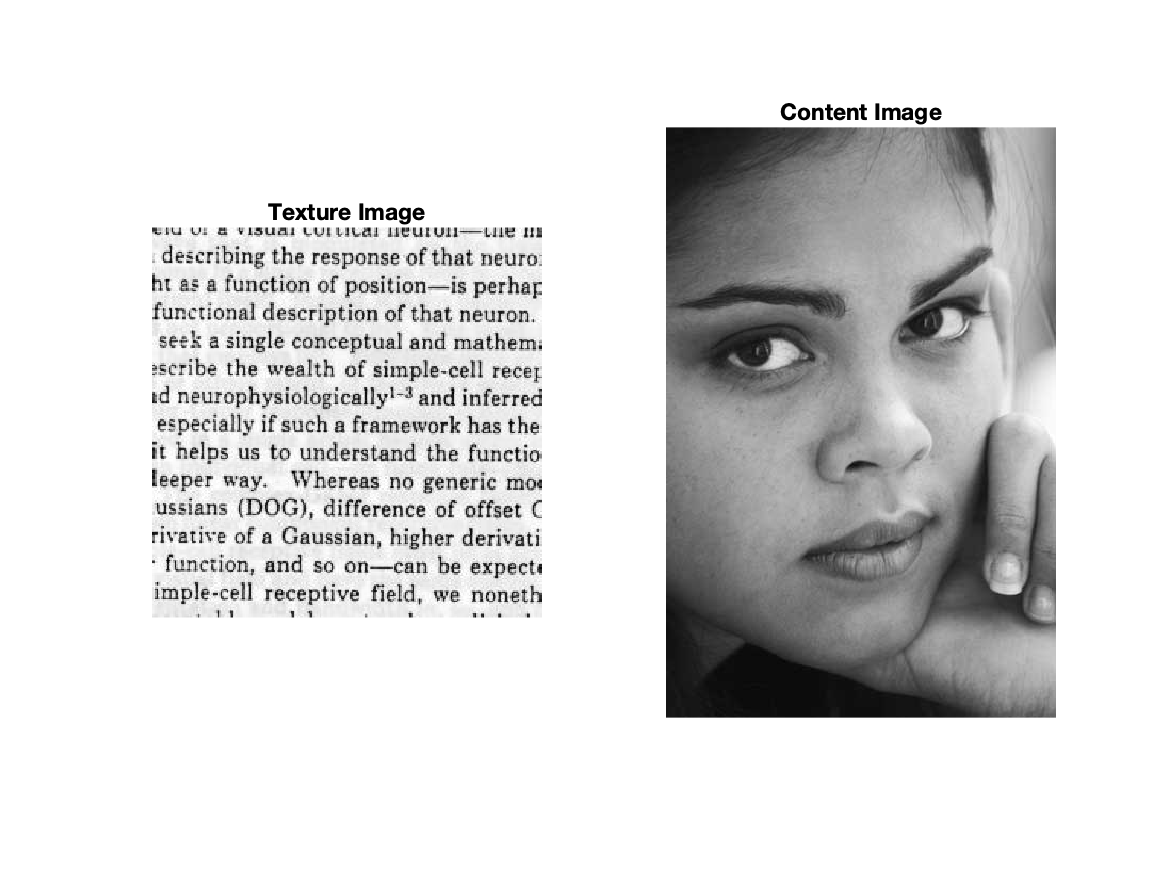
\includegraphics[trim={2cm 4cm 2cm 1cm}, clip, scale=0.5]{../results/bsize/inp_text_girl.png}
        \caption{Input}
    \end{subfigure}
    \hfill
    \begin{subfigure}[h]{0.5\textwidth}
       \centering
       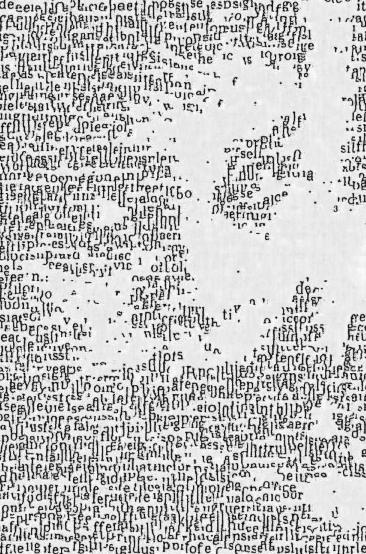
\includegraphics[scale=0.4]{../results/bsize/out_text_girl_B_10_bdr_0_700000.png}`'
       \caption{Output}
   \end{subfigure}
   \caption{Result for texture Text transferred to Girl image}
   \label{fig:ap_bs}
\end{figure*}

\begin{figure*}[h]
    \centering
    \begin{subfigure}[h]{0.45\textwidth}
        \centering
        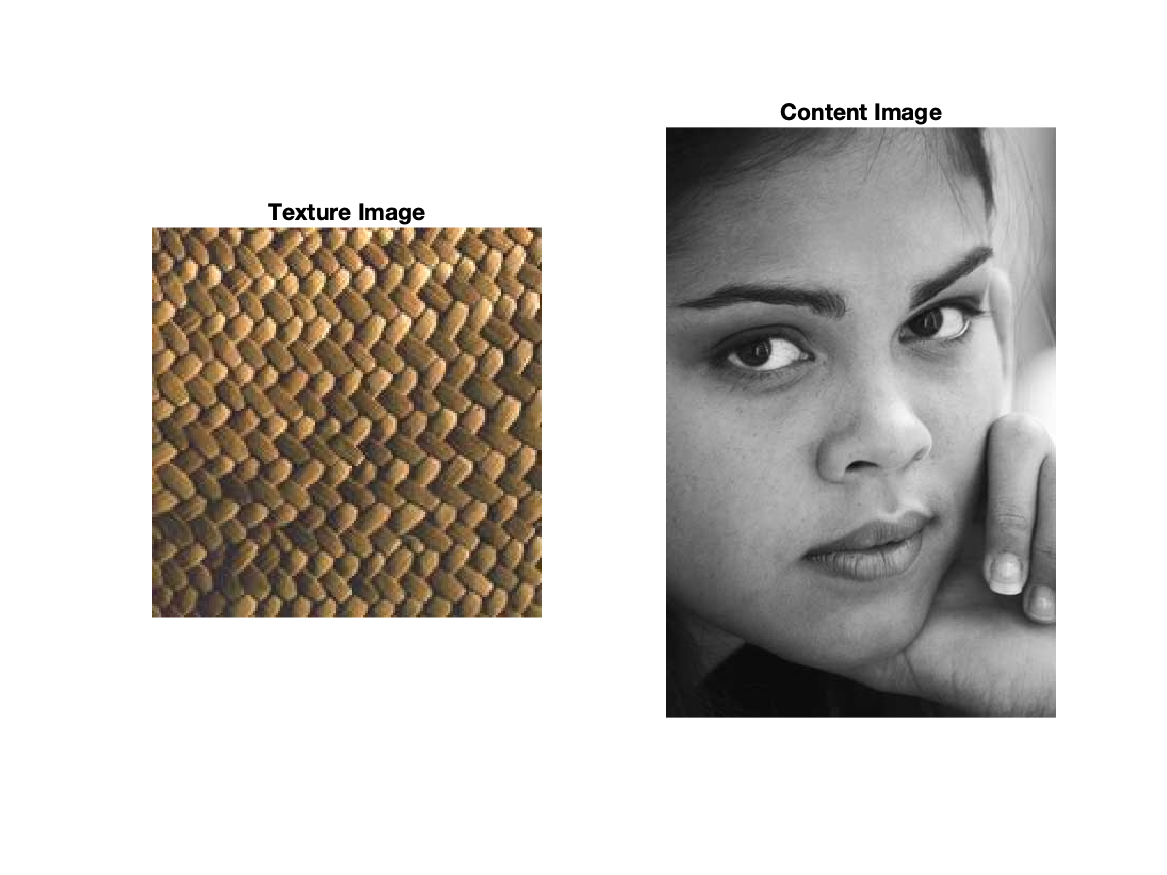
\includegraphics[trim={2cm 4cm 2cm 1cm}, clip, scale=0.5]{../results/bsize/inp_fabric_girl.png}
        \caption{Input}
    \end{subfigure}
    \hfill
    \begin{subfigure}[h]{0.5\textwidth}
       \centering
       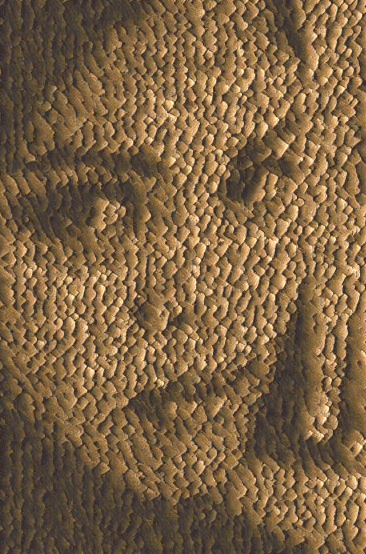
\includegraphics[scale=0.4]{../results/bsize/out_fabric_girl_B_10_bdr_0_800000.png}
       \caption{Output}
   \end{subfigure}
   \caption{Result for texture Fabric transferred to Girl image}
   \label{fig:ap_bs}
\end{figure*}

\begin{figure*}[h]
    \centering
    \begin{subfigure}[h]{0.45\textwidth}
        \centering
        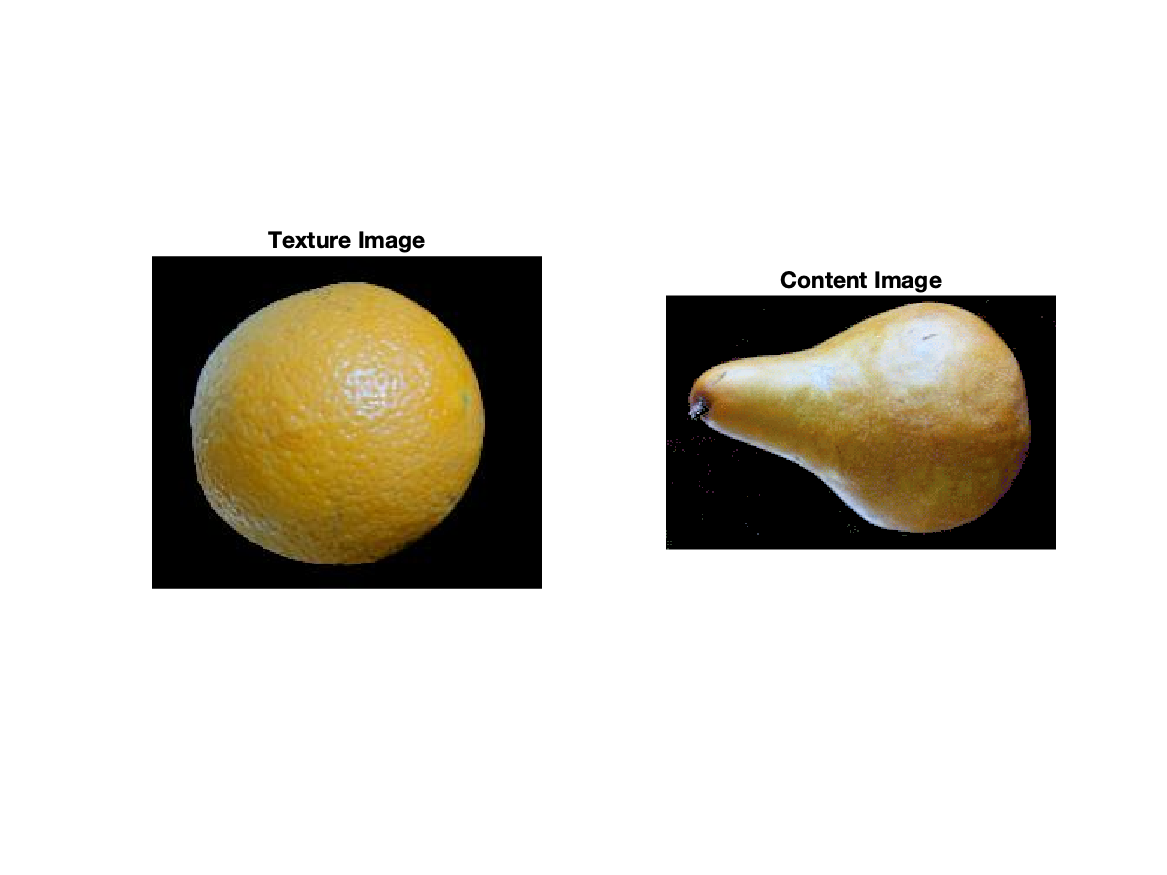
\includegraphics[trim={2cm 4cm 2cm 3cm}, clip, scale=0.5]{../results/bsize/inp_orange_pear.png}
        \caption{Input}
    \end{subfigure}
    \hfill
    \begin{subfigure}[h]{0.5\textwidth}
       \centering
       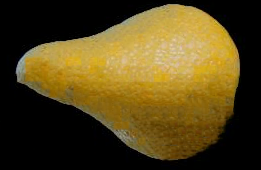
\includegraphics[scale=0.4]{../results/bsize/out_orange_pear_B_20_bdr_0_800000.png}
       \caption{Output}
   \end{subfigure}
   \caption{Result for texture Orange transferred to Pear image}
   \label{fig:ap_bs}
\end{figure*}

\begin{figure*}[h]
    \centering
    \begin{subfigure}[h]{0.45\textwidth}
        \centering
        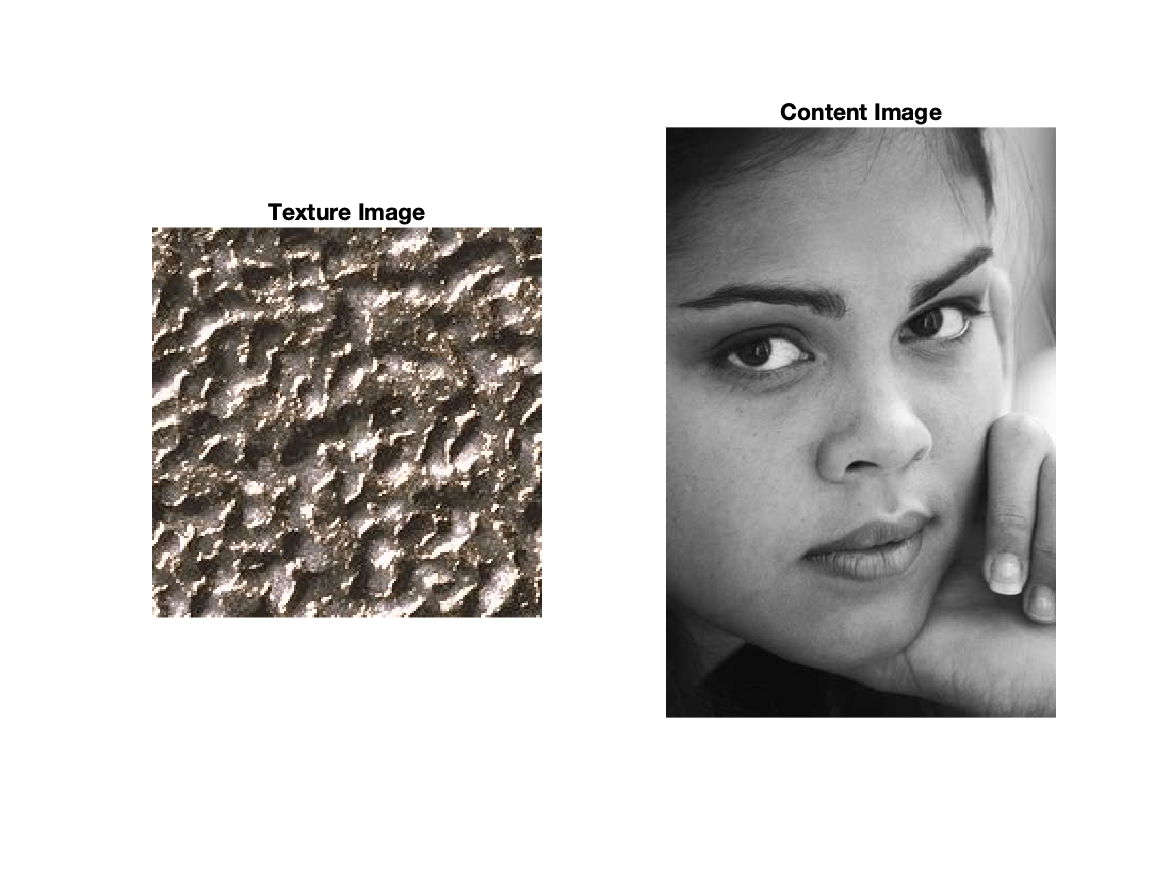
\includegraphics[trim={2cm 4cm 2cm 3cm}, clip, scale=0.5]{../results/bsize/inp_br_pattern_girl.png}
        \caption{Input}
    \end{subfigure}
    \hfill
    \begin{subfigure}[h]{0.5\textwidth}
       \centering
       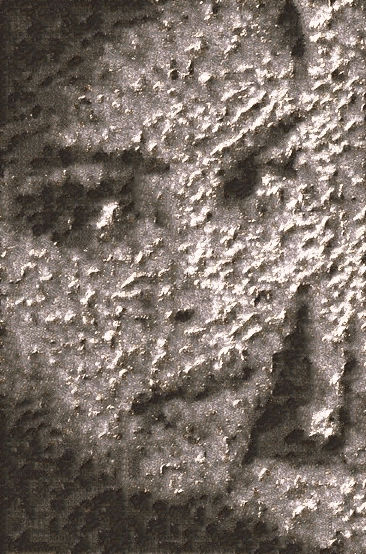
\includegraphics[scale=0.4]{../results/bsize/out_br_pattern_girl_B_10_bdr_0_900000.png}
       \caption{Output}
   \end{subfigure}
   \caption{Result for texture Pattern transferred to Girl image}
   \label{fig:ap_bs}
\end{figure*}
\vspace{-80pt}
% \begin{thebibliography}{999}

% \bibitem{one}
% https://www.geeksforgeeks.org/deep-q-learning/

% \bibitem{two}
% https://www.cs.swarthmore.edu/~bryce/cs63/s16/slides/3-25approximateQ-learning.pdf
% main ref for QL: 
% \bibitem{three}
% http://www.gatsby.ucl.ac.uk/~dayan/papers/cjch.pdf
% \bibitem{four}
% https://courses.cs.washington.edu/courses/cse473/16au/slides-16au/18-approx-rl2.pdf
% \bibitem{five}
% https://www.intel.ai/demystifying-deep-reinforcement-learning/\#gs.hxyudi
% \bibitem{six}
% https://pdfs.semanticscholar.org/2d7e/7d809af7d68c.pdf
% \bibitem{seven}
% https://github.com/moduIo/Deep-Q-network
% \bibitem{eight}
% https://towardsdatascience.com/advanced-dqns-playing-pac-man-with-deep-reinforcement-learning-3ffbd99e0814
% \bibitem{nine}
% {https://lilianweng.github.io/lil-log/2018/05/05/implementing-deep-reinforcement-learning-models.html}
% \bibitem{ten}{https://gym.openai.com/envs/MsPacman-v0/}
% \bibitem{eleven}{https://github.com/gauravmittal1995/Pyman}
% \bibitem{twelve}{https://pythonprogramming.net/pygame-python-3-part-1-intro/}
% \bibitem{thirteen}{https://oregonstate.instructure.com }
% \end{thebibliography}
\clearpage
\section{Ablation Studies}
% Add parameters chosen and values of different things learning rate
\subsection{Quilting}
The effect of block size can be seen in figures \ref{fig:ap_bs}, \ref{fig:cans_bs} and \ref{fig:brick_bs}. As we can see, lower block sizes are not enough to capture the complete texture, hence lead to distorted boundaries and merging of the objects. E.g. consider the apples image, here in the case of B=20, the block size is not large enough to capture a complete apple in the overlapping region, hence in the overlapping region, we can see a lot of apples merging with each other. A very large block size is also not preferable since it reduces the number of patches we select from which means that there is less chance of adjacent patches matching with each other, hence at the boundaries of patches we will observe discontinuity.
\begin{figure*}[h]
    \centering
    \begin{subfigure}[h]{0.2\textwidth}
        \centering
        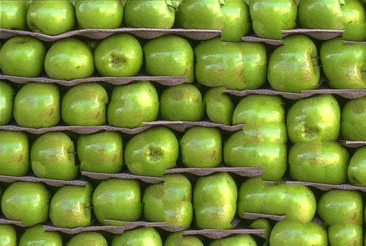
\includegraphics[scale=0.25]{../results/syn/out_apples_B_20.png}
        \caption{B=20}
    \end{subfigure}
    \hfill
    \begin{subfigure}[h]{0.2\textwidth}
       \centering
       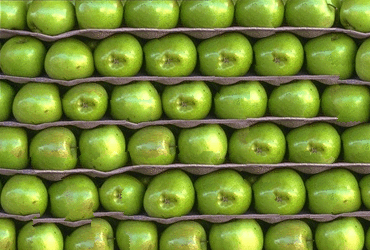
\includegraphics[scale=0.25]{../results/syn/out_apples_B_30.png}
       \caption{B=30}
   \end{subfigure}
   \hfill
   \begin{subfigure}[h]{0.2\textwidth}
       \centering
       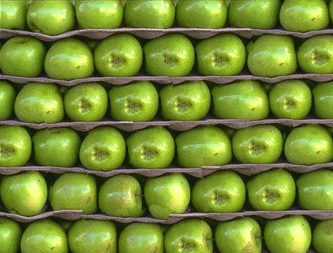
\includegraphics[scale=0.25]{../results/syn/out_apples_B_40.png}
       \caption{B=40}
   \end{subfigure}
   \begin{subfigure}[h]{0.2\textwidth}
       \centering
       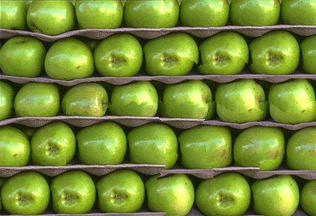
\includegraphics[scale=0.25]{../results/syn/out_apples_B_50.png}
       \caption{B=50}
   \end{subfigure}
   \caption{Effect of block size on Apples}
   \label{fig:ap_bs}
\end{figure*}

\begin{figure*}[h]
    \centering
    \begin{subfigure}[h]{0.2\textwidth}
        \centering
        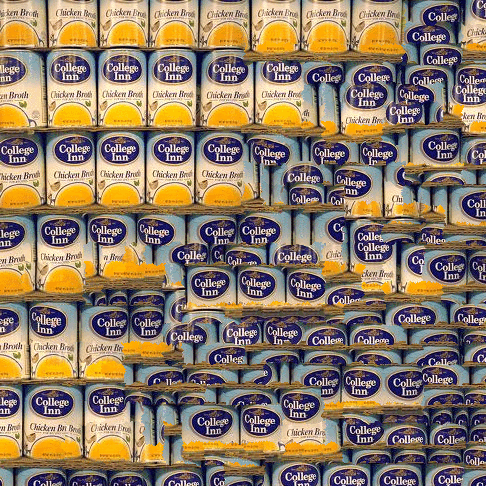
\includegraphics[scale=0.15]{../results/syn/out_cans_B_20.png}
        \caption{B=20}
    \end{subfigure}
    \hfill
    \begin{subfigure}[h]{0.2\textwidth}
       \centering
       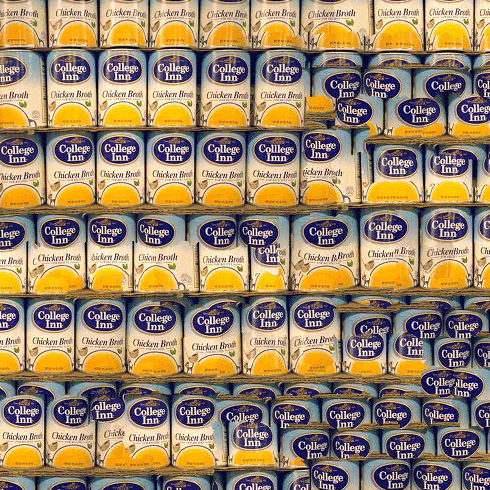
\includegraphics[scale=0.15]{../results/syn/out_cans_B_30.png}
       \caption{B=30}
   \end{subfigure}
   \hfill
   \begin{subfigure}[h]{0.2\textwidth}
       \centering
       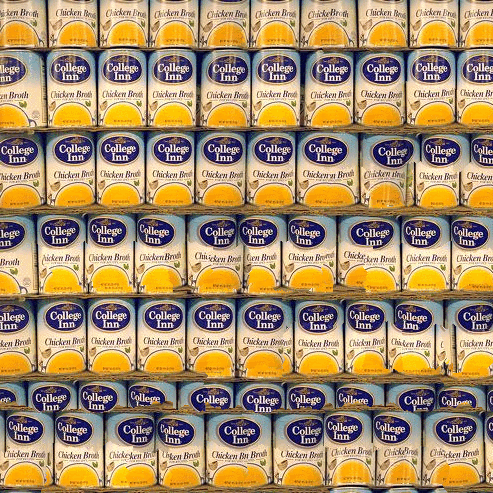
\includegraphics[scale=0.15]{../results/syn/out_cans_B_40.png}
       \caption{B=40}
   \end{subfigure}
   \begin{subfigure}[h]{0.2\textwidth}
       \centering
       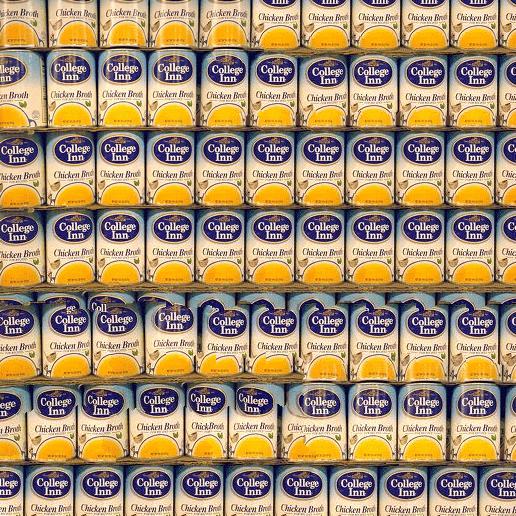
\includegraphics[scale=0.15]{../results/syn/out_cans_B_50.png}
       \caption{B=50}
   \end{subfigure}
   \caption{Effect of block size on Cans}
   \label{fig:cans_bs}
\end{figure*}

\begin{figure*}[h]
    \centering
    \begin{subfigure}[h]{0.2\textwidth}
        \centering
        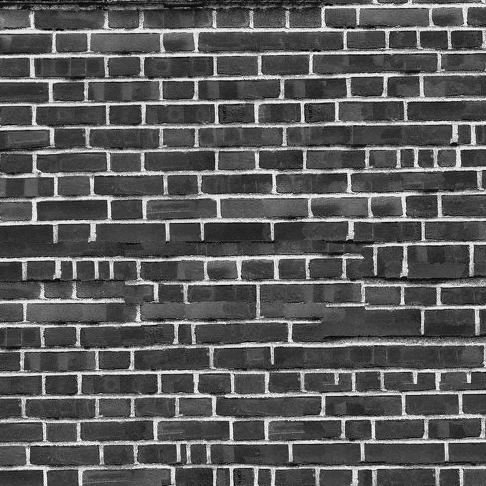
\includegraphics[scale=0.15]{../results/syn/out_brick_bw_B_20.png}
        \caption{B=20}
    \end{subfigure}
    \hfill
    \begin{subfigure}[h]{0.2\textwidth}
       \centering
       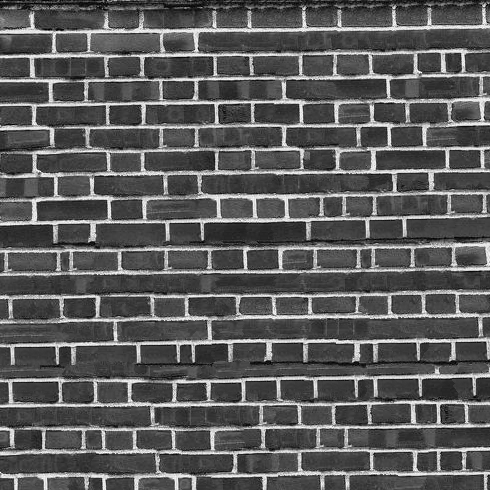
\includegraphics[scale=0.15]{../results/syn/out_brick_bw_B_30.png}
       \caption{B=30}
   \end{subfigure}
   \hfill
   \begin{subfigure}[h]{0.2\textwidth}
       \centering
       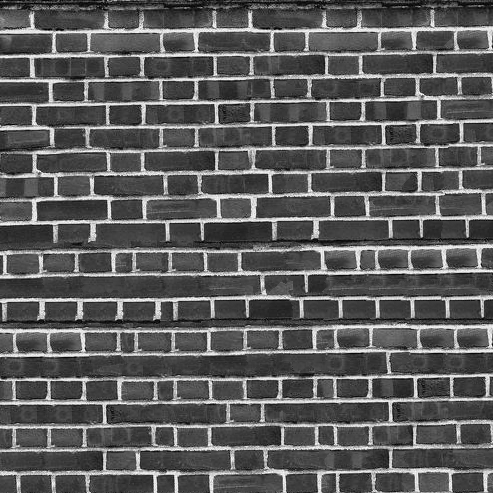
\includegraphics[scale=0.15]{../results/syn/out_brick_bw_B_40.png}
       \caption{B=40}
   \end{subfigure}
   \begin{subfigure}[h]{0.2\textwidth}
       \centering
       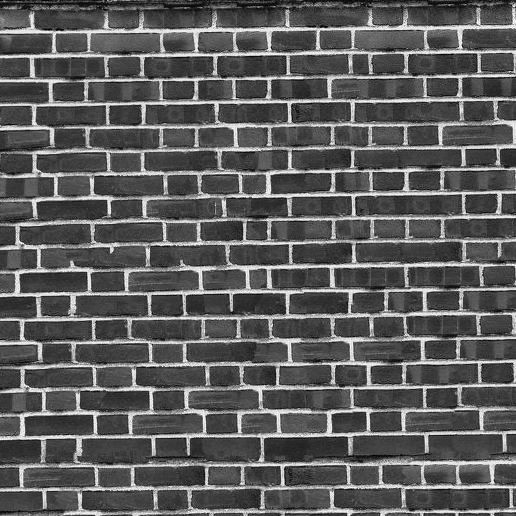
\includegraphics[scale=0.15]{../results/syn/out_brick_bw_B_50.png}
       \caption{B=50}
   \end{subfigure}
   \caption{Effect of block size on Bricks}
   \label{fig:brick_bs}
\end{figure*}

% \begin{table}[!th]
% \begin{center}
% \begin{tabular}{|l|c|}
% \hline
% Situation & Reward \\
% \hline\hline
% Win (finish food) & +500 \\
% Lose (eaten by ghost) & -500 \\
% Eat food & +10\\
% Consume ghost & +200\\
% Idle/no food & -1\\
% \hline
% \end{tabular}
% \end{center}
% \caption{Game parameters for Q-Learning}
% \end{table}
% The features chosen for training the Approximate Q-Learning Network are: bias, number\_of\_ghosts\_1\_step\_away, distance\_to\_closest\_food
% \begin{table}[!th]
% \begin{center}
% \begin{tabular}{|l|c|c|c|c|}
% \hline
% Approach & Grid size & Avg Score & \#Epochs & Time (train)\\
% \hline\hline
% AQL & mediumClassic & 1202.7 & 50 & 5m 45s\\
% AQL & mediumGrid & 526.4 & 50 & 32s \\
% QL & smallGrid & 499.5 & 2000 & 1m 24s\\
% \hline
% \end{tabular}
% \end{center}
% \caption{Some simulations}
% \label{tab:qlres}
% \end{table}


% \begin{figure}[h]
% \begin{center}
% 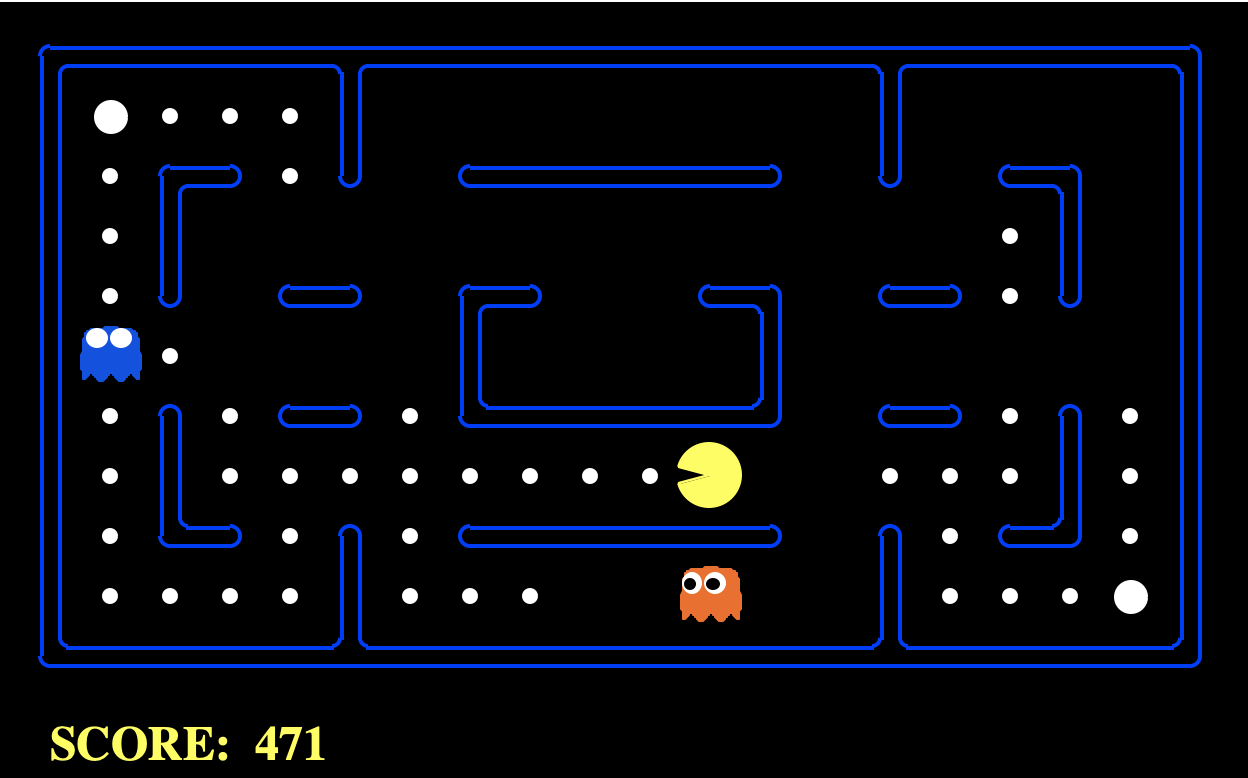
\includegraphics[scale=0.25]{resources/game_preview.png}
% \end{center}
% \vspace{-0.2em}
% \caption{Pac-Man during Training}
% \label{fig:basic}
% \end{figure}
\clearpage
\subsection{Transfer}
Here, we study the effect of changing block size on the texture transfer result. When the block size is small, content preservation is more because the overlapping region more accurately represents the approximate intensity of the complete block hence matching that leads to a result which closely resembles the target image content. However, a small block size is not enough to capture the complete texture of the image as we saw in texture synthesis, hence the texture of the image is better preserved when the block size is larger. Hence, there is a tradeoff between content preservation and texture preservation and hence the block size must be tuned appropriately to get visually pleasing results.

We also study the output images obtained after each iteration of the algorithm. In the earlier iterations, a small value of $\alpha_{i}$ is used which means that the content preservation will be more but there will be some artifacts in the boundary of the patches and the texture will not be very clear. This is because the error weight given to matching the overlapping region with the previously places blocks is low, hence we will observe discontinuity in the edges of the patches. As we reach the later iterations, this quantity $\alpha_{i}$ is gradually increased which removes these boundary artifacts and leads to a better image texture and continuity while sacrificing a bit on the content preservation. Hence, the number of iterations must also be tuned properly for superior results.
\begin{figure*}[h]
    \begin{center}
    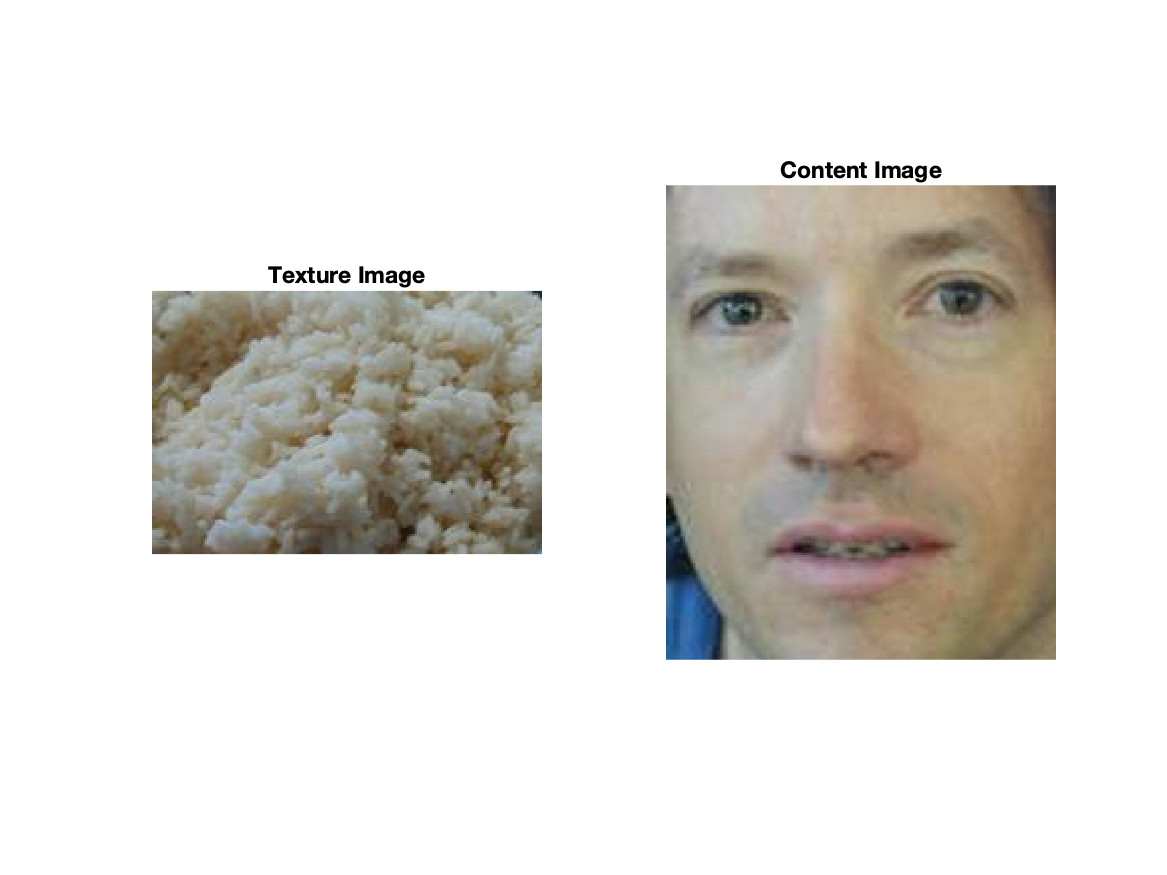
\includegraphics[trim={2cm 4cm 2cm 2cm}, clip, scale=0.5]{../results/bsize/inp_rice_bill.png}
    \end{center}
    \vspace{-0.2em}
    \caption{Rice-Bill input}
    \label{fig:rice_bill}
\end{figure*}

% Block Size
\begin{figure*}[h]
    \begin{center}
    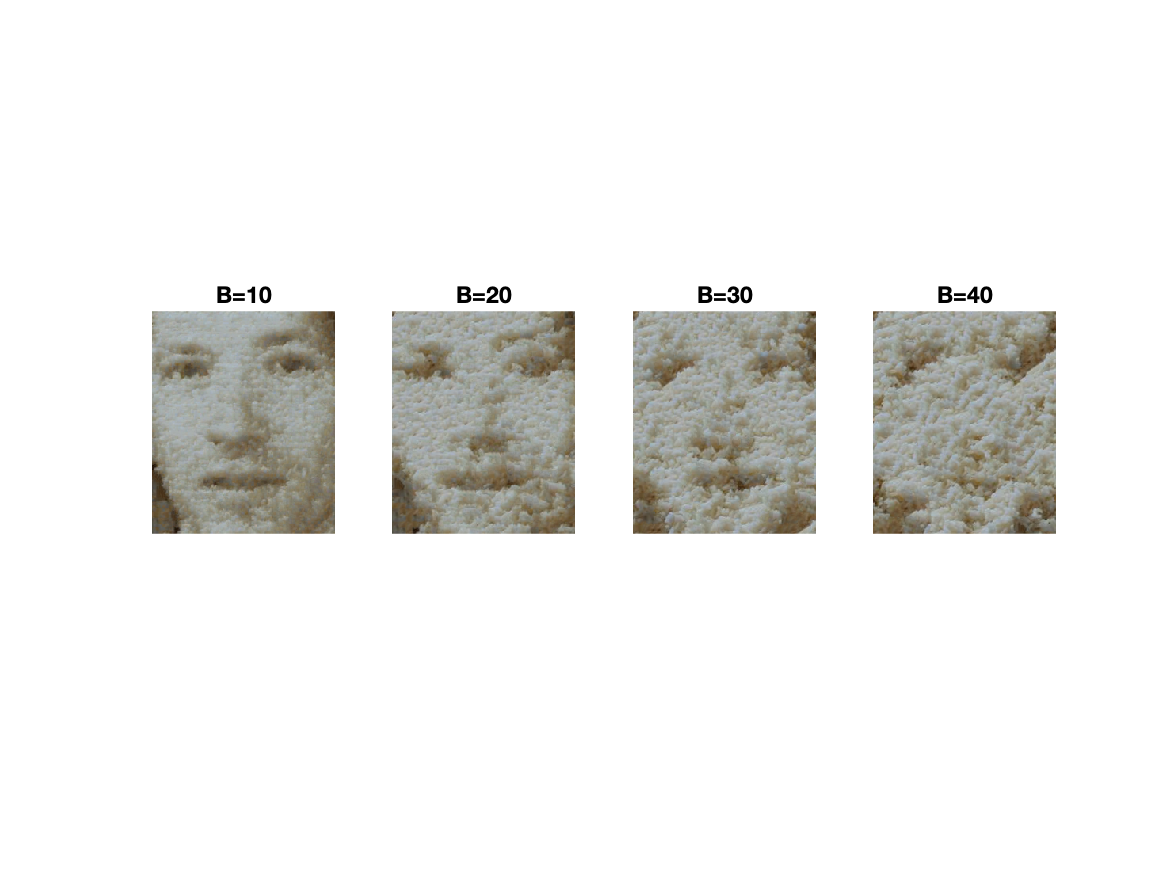
\includegraphics[trim={2cm 6cm 2cm 4cm}, clip, scale=0.9]{../results/bsize/res_rice_bill_bdr_0_800000_iter_5.png}
    \end{center}
    \vspace{-0.2em}
    \caption{Rice-Bill, Block Size, B decay rate = 0.8}
    \label{fig:rice_bill_bs}
\end{figure*}

% Changes with iteration
\begin{figure*}[h]
    \begin{center}
    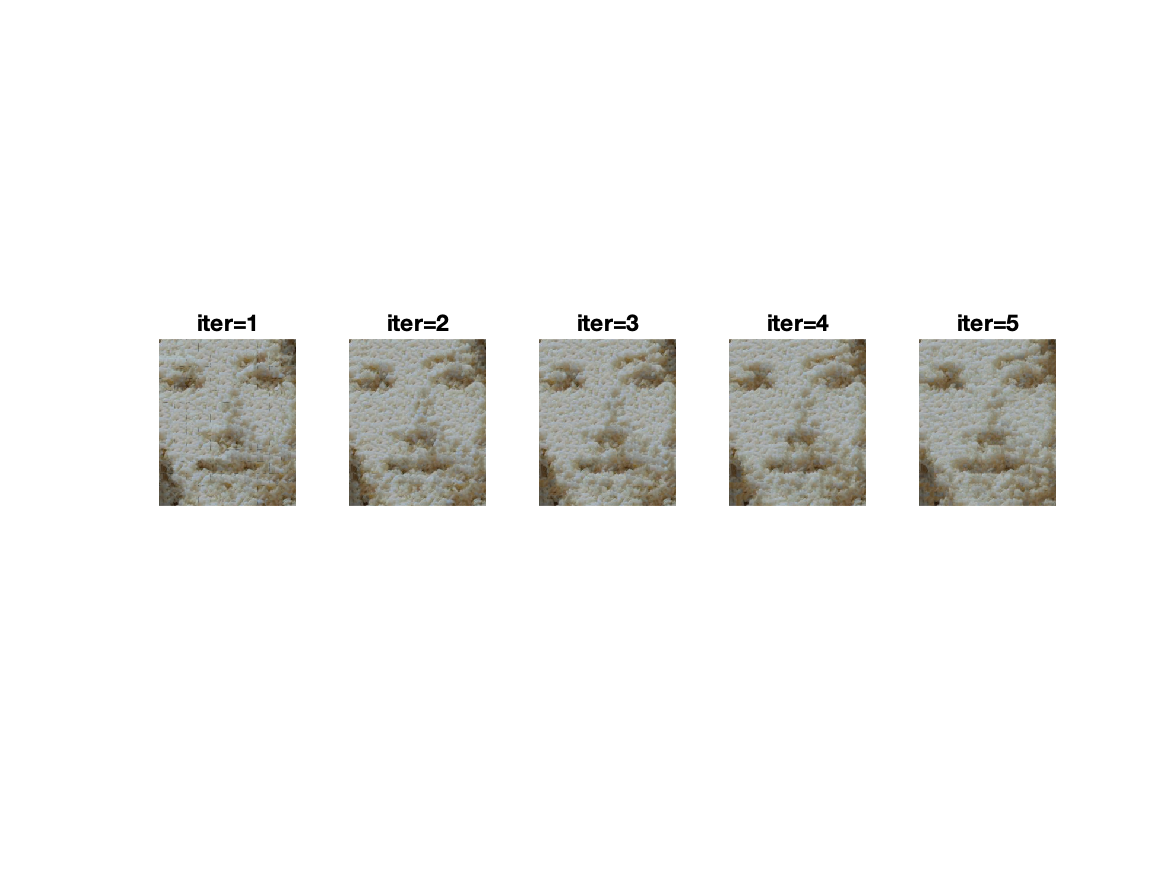
\includegraphics[trim={2cm 6cm 2cm 4cm}, clip, scale=0.9]{../results/iters/res_rice_bill_b_20_bdr_0_800000.png}
    \end{center}
    \vspace{-0.2em}
    \caption{Rice-Bill, Iterations, Block size=20, B decay rate = 0.8}
    \label{fig:rice_bill_iter}
\end{figure*}

\begin{figure*}[h]
    \begin{center}
    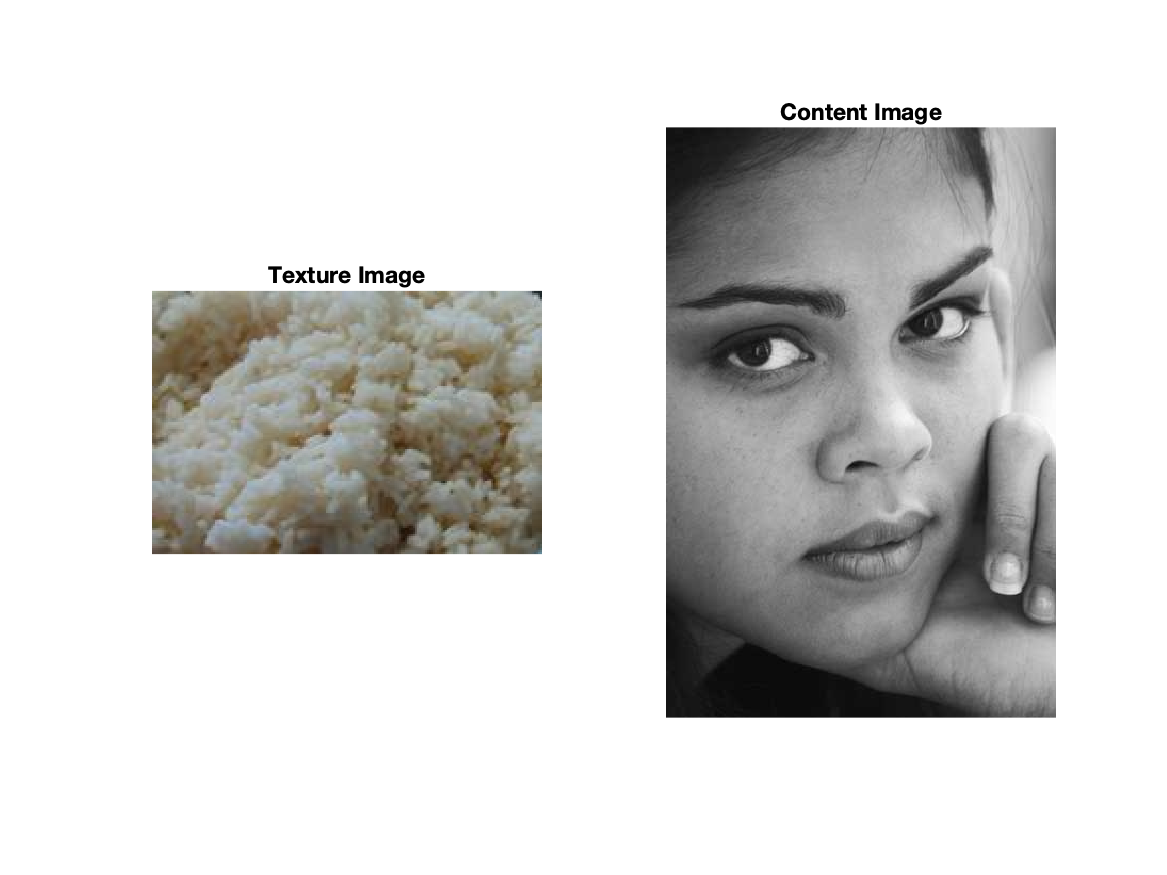
\includegraphics[trim={2cm 4cm 2cm 2cm}, clip, scale=0.5]{../results/bsize/inp_rice_girl.png}
    \end{center}
    \vspace{-0.2em}
    \caption{Rice-Girl input}
    \label{fig:rice_girl}
\end{figure*}

\begin{figure*}[h]
    \begin{center}
    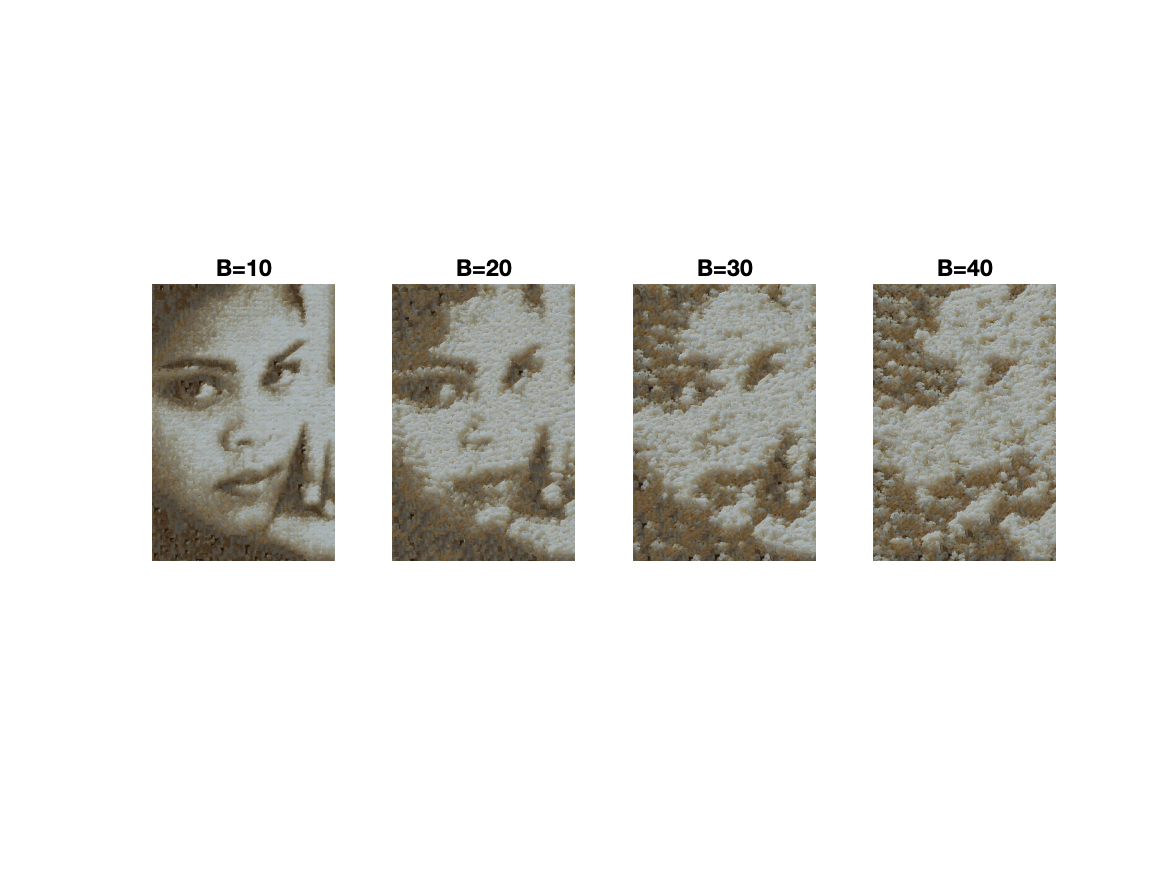
\includegraphics[trim={2cm 6cm 2cm 4cm}, clip, scale=0.9]{../results/bsize/res_rice_girl_bdr_0_700000_iter_5.png}
    \end{center}
    \vspace{-0.2em}
    \caption{Rice-Girl, Block Size, B decay rate = 0.7}
    \label{fig:rice_girl_bs}
\end{figure*}

% Changes with iteration
\begin{figure*}[h]
    \begin{center}
    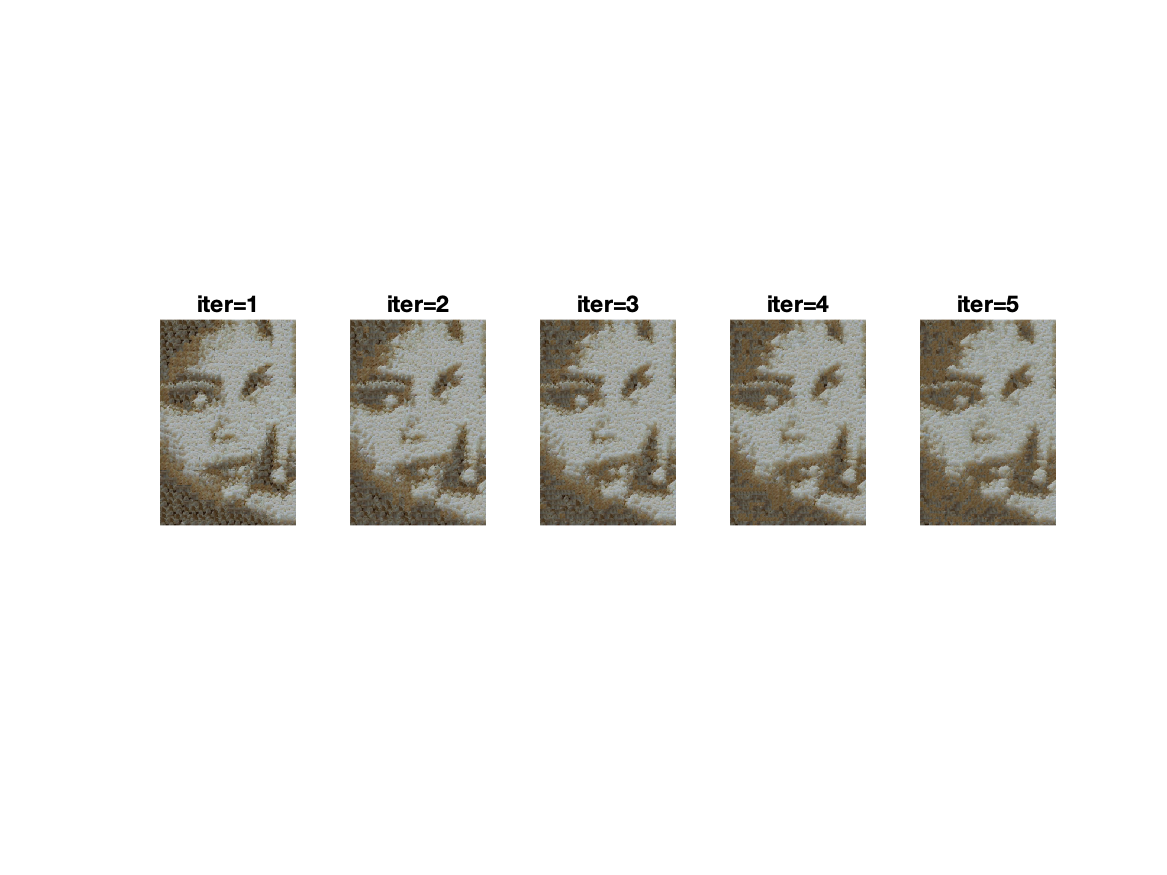
\includegraphics[trim={2cm 6cm 2cm 4cm}, clip, scale=0.9]{../results/iters/res_rice_girl_b_20_bdr_0_800000.png}
    \end{center}
    \vspace{-0.2em}
    \caption{Rice-Girl, Iterations, Block size=20, B decay rate = 0.8}
    \label{fig:rice_girl_iter}
\end{figure*}


\begin{figure*}[h]
    \begin{center}
    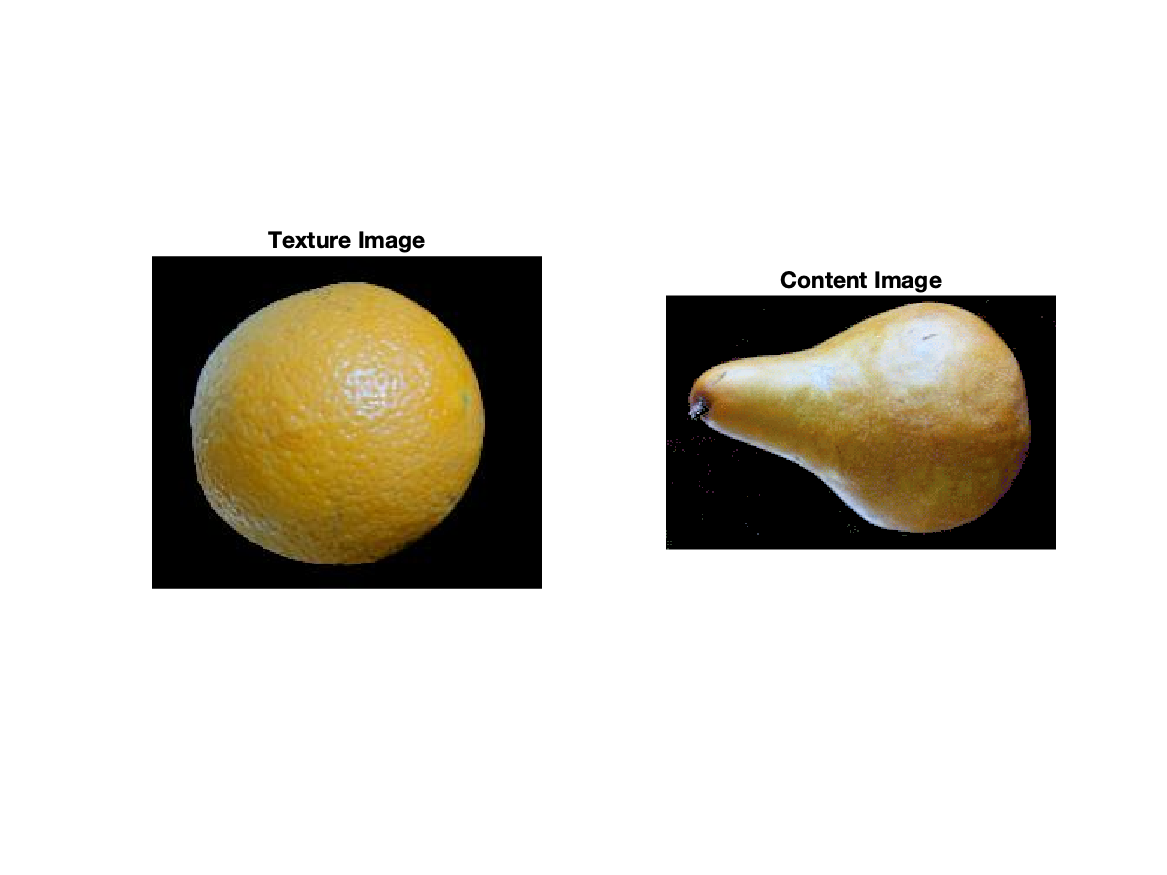
\includegraphics[trim={2cm 4cm 2cm 2cm}, clip, scale=0.5]{../results/bsize/inp_orange_pear.png}
    \end{center}
    \vspace{-0.2em}
    \caption{Orange-Pear input}
    \label{fig:or_pear}
\end{figure*}

\begin{figure*}[h]
    \begin{center}
    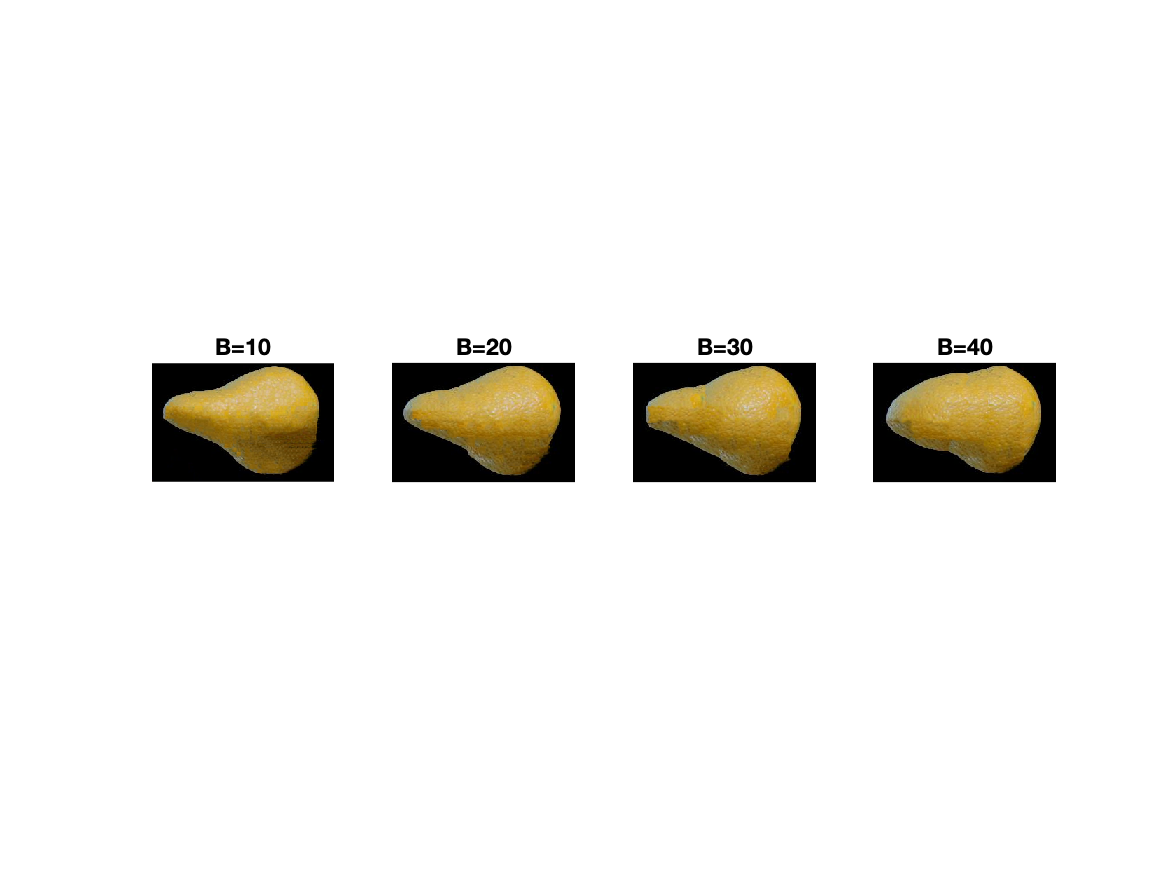
\includegraphics[trim={2cm 6cm 2cm 4cm}, clip, scale=0.9]{../results/bsize/res_orange_pear_bdr_0_900000_iter_5.png}
    \end{center}
    \vspace{-0.2em}
    \caption{Orange-Pear, Block Size, B decay rate = 0.9}
    \label{fig:orange_pear_bs}
\end{figure*}

% Changes with iteration
\begin{figure*}[h]
    \begin{center}
    \includegraphics[trim={2cm 6cm 2cm 4cm}, clip, scale=0.9]{../results/iters/res_orange_pear_b_20_bdr_0_800000.png}
    \end{center}
    \vspace{-0.2em}
    \caption{Orange-Pear, Iterations, Block size=20, B decay rate = 0.8}
    \label{fig:or_pear_iter}
\end{figure*}

\end{document}